\documentclass[12pt]{article}
% --------------------------------------------------------------
% This is all preamble stuff that you don't have to worry about.
% Head down to where it says "Start here"
% --------------------------------------------------------------

\usepackage[margin=1in]{geometry} 
\usepackage{amsmath,amsthm,amssymb}
\usepackage[margin=1in]{geometry} 
\usepackage{amsmath,amsthm,amssymb}
\usepackage[english]{babel} %Castellanización
\usepackage[T1]{fontenc} %escribe lo del teclado
\usepackage[utf8]{inputenc} %Reconoce algunos símbolos
\usepackage{lmodern} %optimiza algunas fuentes
\usepackage{graphicx}
%\graphicspath{ {images/} }
%\usepackage{apacite} 
\usepackage{mathtools}
\DeclarePairedDelimiter\bra{\langle}{\rvert}
\DeclarePairedDelimiter\ket{\lvert}{\rangle}
\DeclarePairedDelimiterX\braket[2]{\langle}{\rangle}{#1 \delimsize\vert #2}
\usepackage{mathrsfs}
\usepackage{amsmath}
\usepackage{xcolor}
\usepackage{lmodern} %optimiza algunas fuentes
\usepackage{titling} % Enables \subtitle command
\usepackage{subfig}
%\usepackage{hyperref}
\usepackage[natbibapa]{apacite} % Load apacite with natbib compatibility
\bibliographystyle{apacite}     % APA citation style
\usepackage{float}
\usepackage{parskip}           % Adds spacing between paragraphs
\usepackage{indentfirst} 
\setlength{\parindent}{1cm}  % Custom indent size (default: 15pt)

\newcommand{\N}{\mathbb{N}}
\newcommand{\Z}{\mathbb{Z}}
 
\newenvironment{theorem}[2][Theorem]{\begin{trivlist}
\item[\hskip \labelsep {\bfseries #1}\hskip \labelsep {\bfseries #2.}]}{\end{trivlist}}
\newenvironment{lemma}[2][Lemma]{\begin{trivlist}
\item[\hskip \labelsep {\bfseries #1}\hskip \labelsep {\bfseries #2.}]}{\end{trivlist}}
\newenvironment{exercise}[2][Exercise]{\begin{trivlist}
\item[\hskip \labelsep {\bfseries #1}\hskip \labelsep {\bfseries #2.}]}{\end{trivlist}}
\newenvironment{problem}[2][Problem]{\begin{trivlist}
\item[\hskip \labelsep {\bfseries #1}\hskip \labelsep {\bfseries #2.}]}{\end{trivlist}}
\newenvironment{question}[2][Question]{\begin{trivlist}
\item[\hskip \labelsep {\bfseries #1}\hskip \labelsep {\bfseries #2.}]}{\end{trivlist}}
\newenvironment{corollary}[2][Corollary]{\begin{trivlist}
\item[\hskip \labelsep {\bfseries #1}\hskip \labelsep {\bfseries #2.}]}{\end{trivlist}}

\newenvironment{solution}{\begin{proof}[Solution]}{\end{proof}}

\usepackage{hyperref} % Uso de links

\usepackage{caption}
\usepackage{subcaption}
\usepackage{subfig}

 
\begin{document}
 
% --------------------------------------------------------------
%                         Start here
% --------------------------------------------------------------
%\color{blue}

\title{Introduction to High Temperature Materials}
\author{Problem Set 4\\
Cap Morales, Shannon Nazareth\\
N25MA13}

\maketitle


\section{}

\subsection{Ni-Al system plotted using Thermo-Calc}

% First part
\begin{figure}[h]
    \centering
    \subfloat[Binary Ni-Al ASM Materials Handbook \label{fig:diagrama_ejemplo}]{
        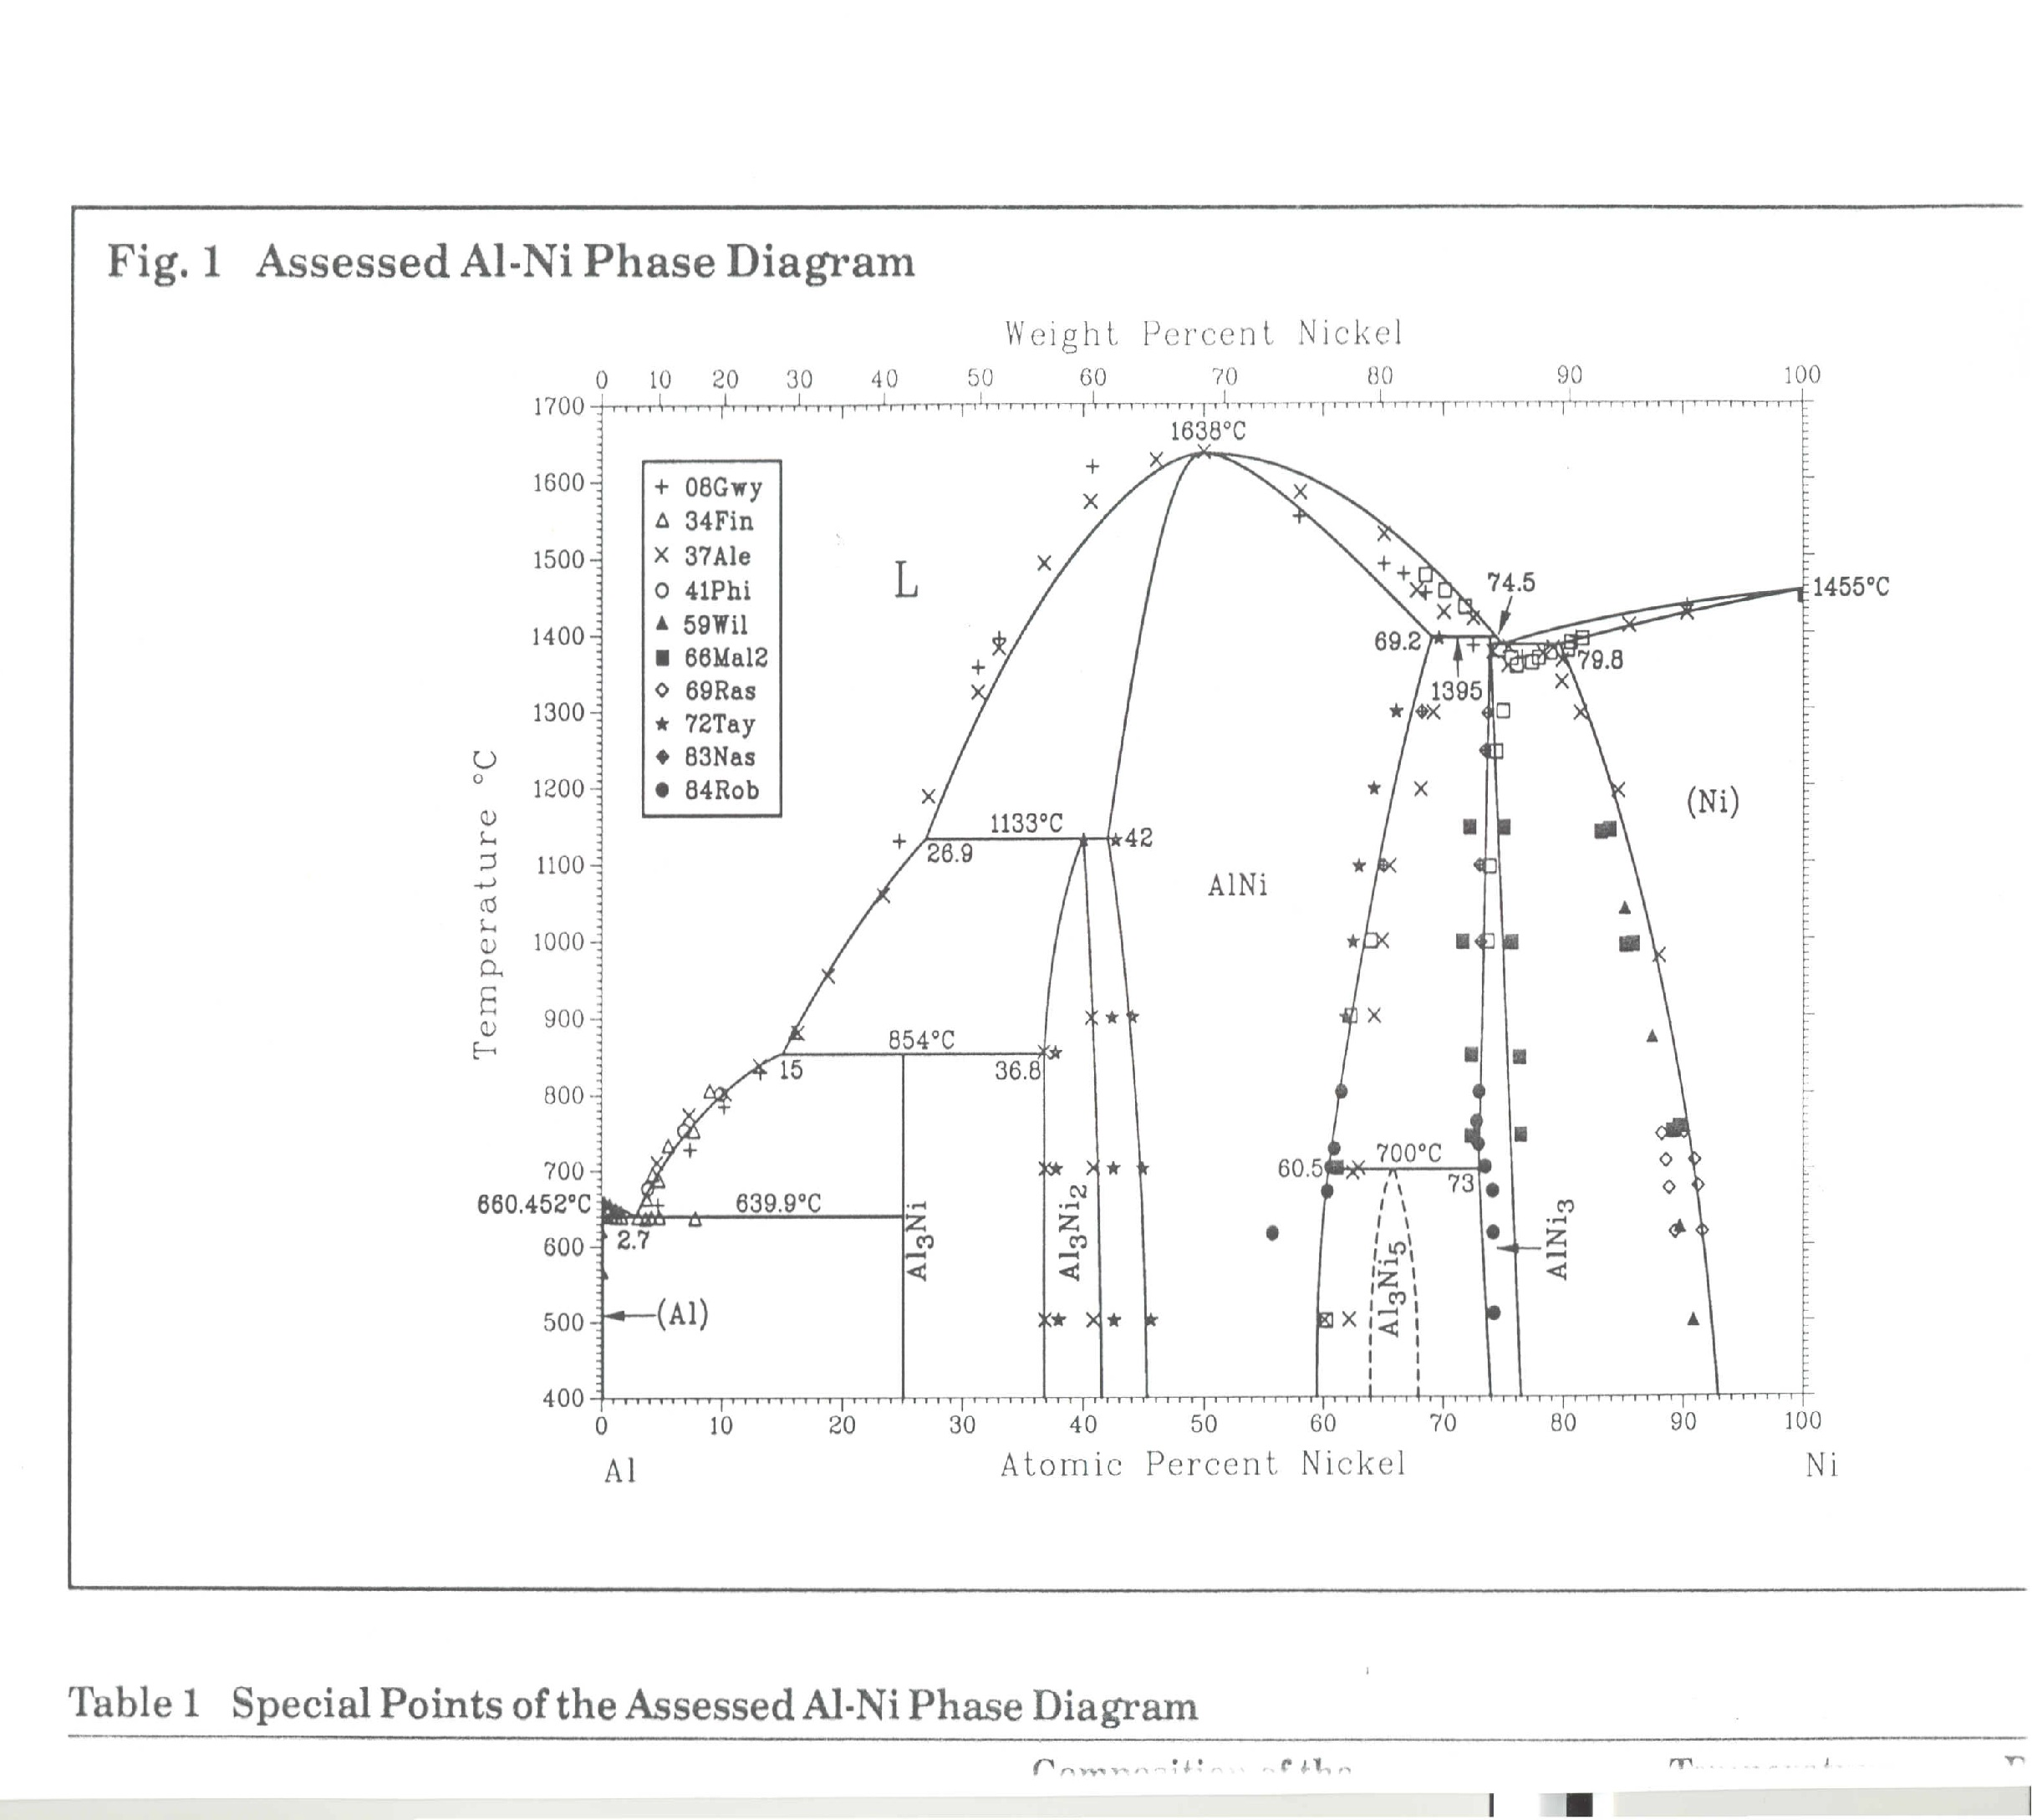
\includegraphics[width=0.85\textwidth]{graficas/diagrama_base.jpg}
        }
        \caption{Ni-Al binary phase diagram}
    \label{fig:Ni-Al_binarydiagram}
\end{figure}
% Second part (automatically continues numbering)
\begin{figure}[h]
    \centering
    \ContinuedFloat % This is the key command
    \subfloat[\centering Ni-Al system obtained using \textit{ThermoCalc} \citep{thermocalc} \label{fig:diagrama01}]{
        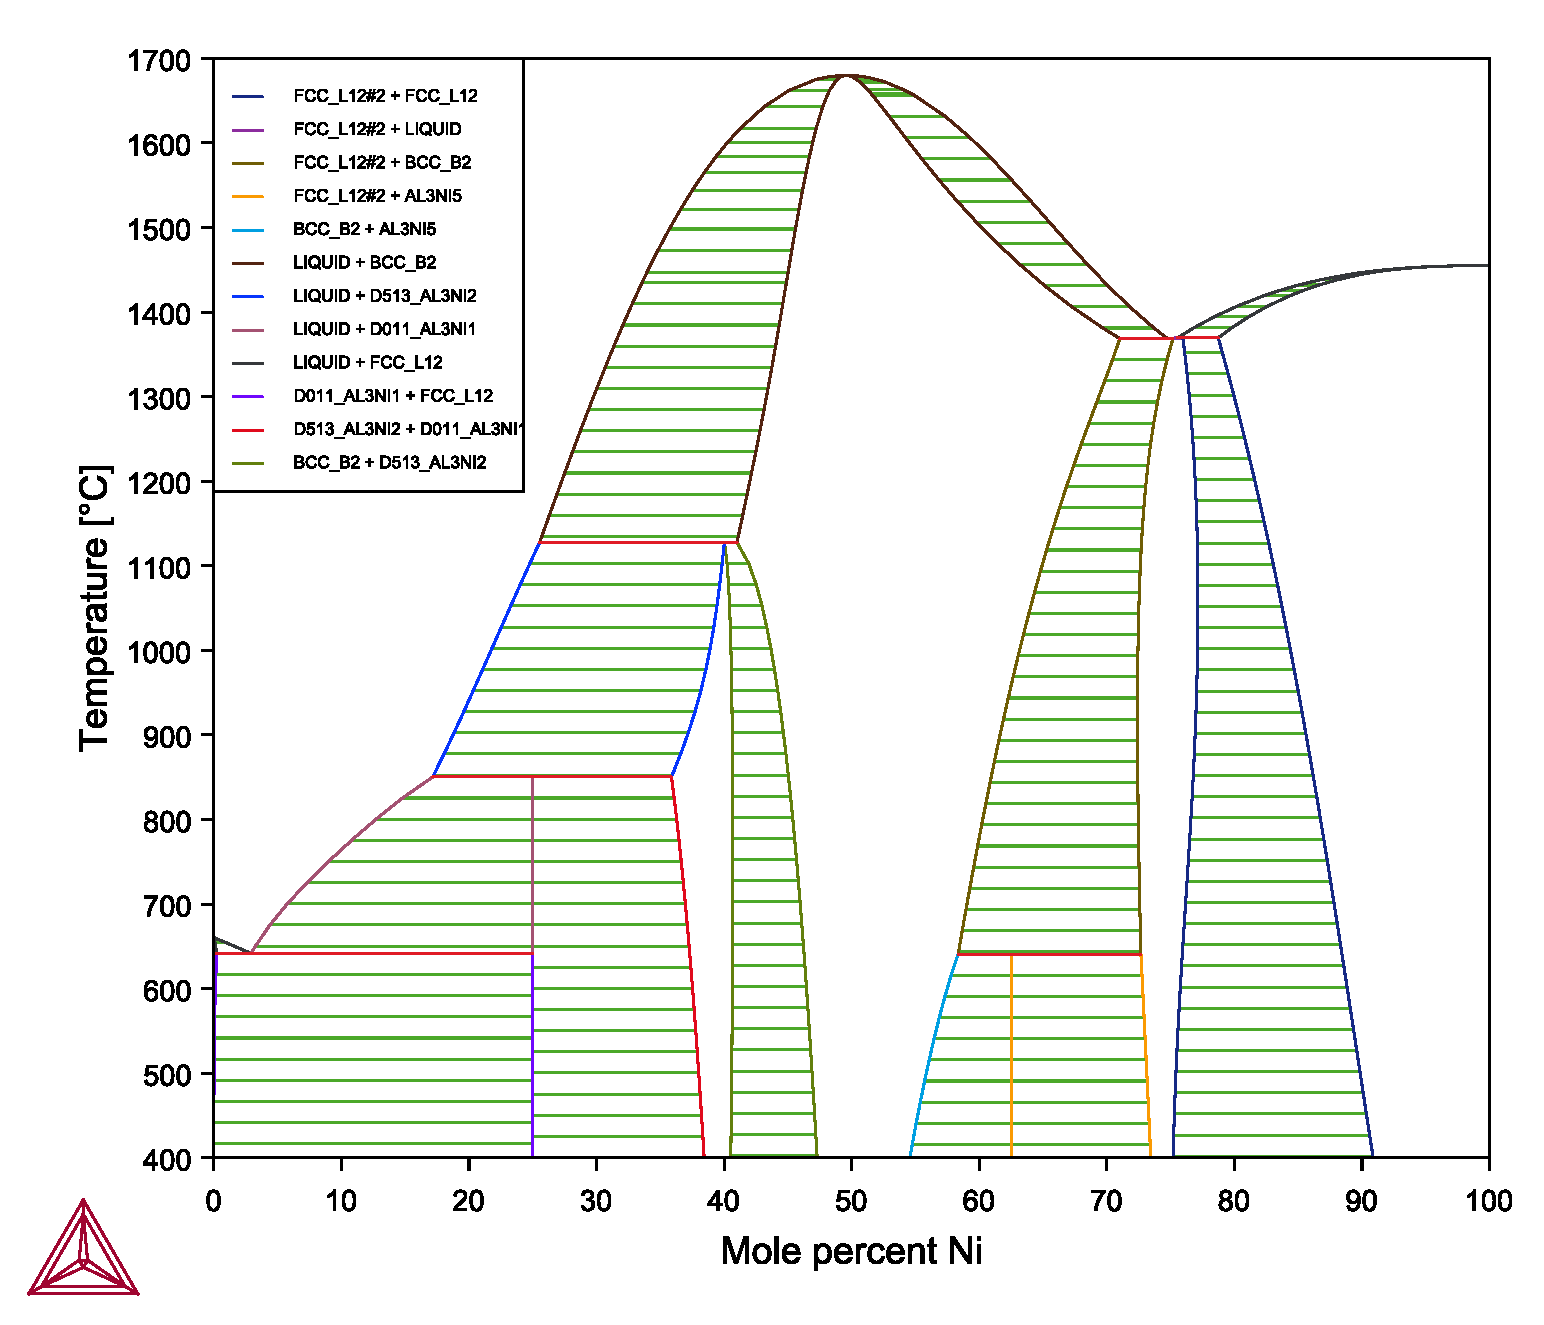
\includegraphics[width=0.9\textwidth]{graficas/Q1_NI_Al_binarydiagram.pdf}
        }
        \caption[]{Ni-Al binary phase diagram (continued)}
\end{figure}

In figure \ref{fig:Ni-Al_binarydiagram} the plots for the binary system of Ni-Al is presented. Figure \ref{fig:diagrama_ejemplo} presents the binary phase diagram from the ASM Materials Handbook; and figure \ref{fig:diagrama01} presents the Ni-Al binary diagram obtained using \textit{ThermoCalc}, using the binary calculator tool.

\newpage
\subsection{Composition of Al in Ni-Al system for a $\gamma'$ fraction is $75\%$. Target operating temperature $1000^{\circ}$C}

The composition of the $\gamma'$ phase was calculated using the single point tool in \textit{ThermoCalc}, from which the following results were obtained:

\begin{table}[H]
    \centering
    \begin{tabular}{lrrr}
        \multicolumn{1}{c}{\textbf{Property}} & \multicolumn{1}{c}{\textbf{Value}} \\ \hline \hline
        Moles & 1 \\ 
        Mass (g) & 51.9841 \\ 
        Temperature (K) & 1273.15 \\ 
        Total Gibbs Energy (J) & -94721.9 \\
        Enthalpy (J) & -2475.10 \\
        Volume (m\textsuperscript{3}) & 0 \\ \\
        \multicolumn{1}{c}{\textbf{Component}} & \multicolumn{1}{c}{\textbf{Mole Fraction}} & \multicolumn{1}{c}{\textbf{Mass Fraction}} & \multicolumn{1}{c}{\textbf{Activity}}\\ \hline \hline
        Al & 0.211490 & 0.109773 & 1.13944E-08 \\
        Ni & 0.788510 & 0.890227 & 0.00159239
    \end{tabular}
    \caption{Results obtained from the calculation of the composition of the Ni-Al system for a $\gamma'$ phase at $75\%$ using \textit{ThermoCalc} \citep{thermocalc}}
    \label{tab:tab01}
\end{table}

From table \ref{tab:tab01} it can be seen that for the $\gamma'$ wit a fraction of $75\%$ at $1000^{\circ}$C the composition for Al is $0.2115$ ($21.15\%$) mole fraction which is equivalent to a $10.98$ weight percent.
\newpage
\section{}

\subsection{Examine the Ni-Al-Ta ternary phase diagram, is there a strong temperature dependence?}

To evaluate if there is a strong dependence on temperature, the Ni-Al-Ta ternary phase diagram was generated using the \textit{phase diagram} tool at different temperatures, from $800^{\circ}$C to $1300^{\circ}$C, the resulting diagrams are shown in figure \ref{fig:diagram02}.

Figures \ref{fig:800C} and \ref{fig:900C} present the ternary phase diagram for the alloy at $800$°C and $900$°C respectively, from the diagrams it can be seen a small increase in the $\gamma$ phase  region. This can be noted in the $\gamma$ boundary line that moves from a mole percent of $12\%$ in figure \ref{fig:800C}, to approximately $14\%$ in the Al axis in figure \ref{fig:900C}.

\begin{figure}[h]
  \centering
  \subfloat[800°C\label{fig:800C}]{
    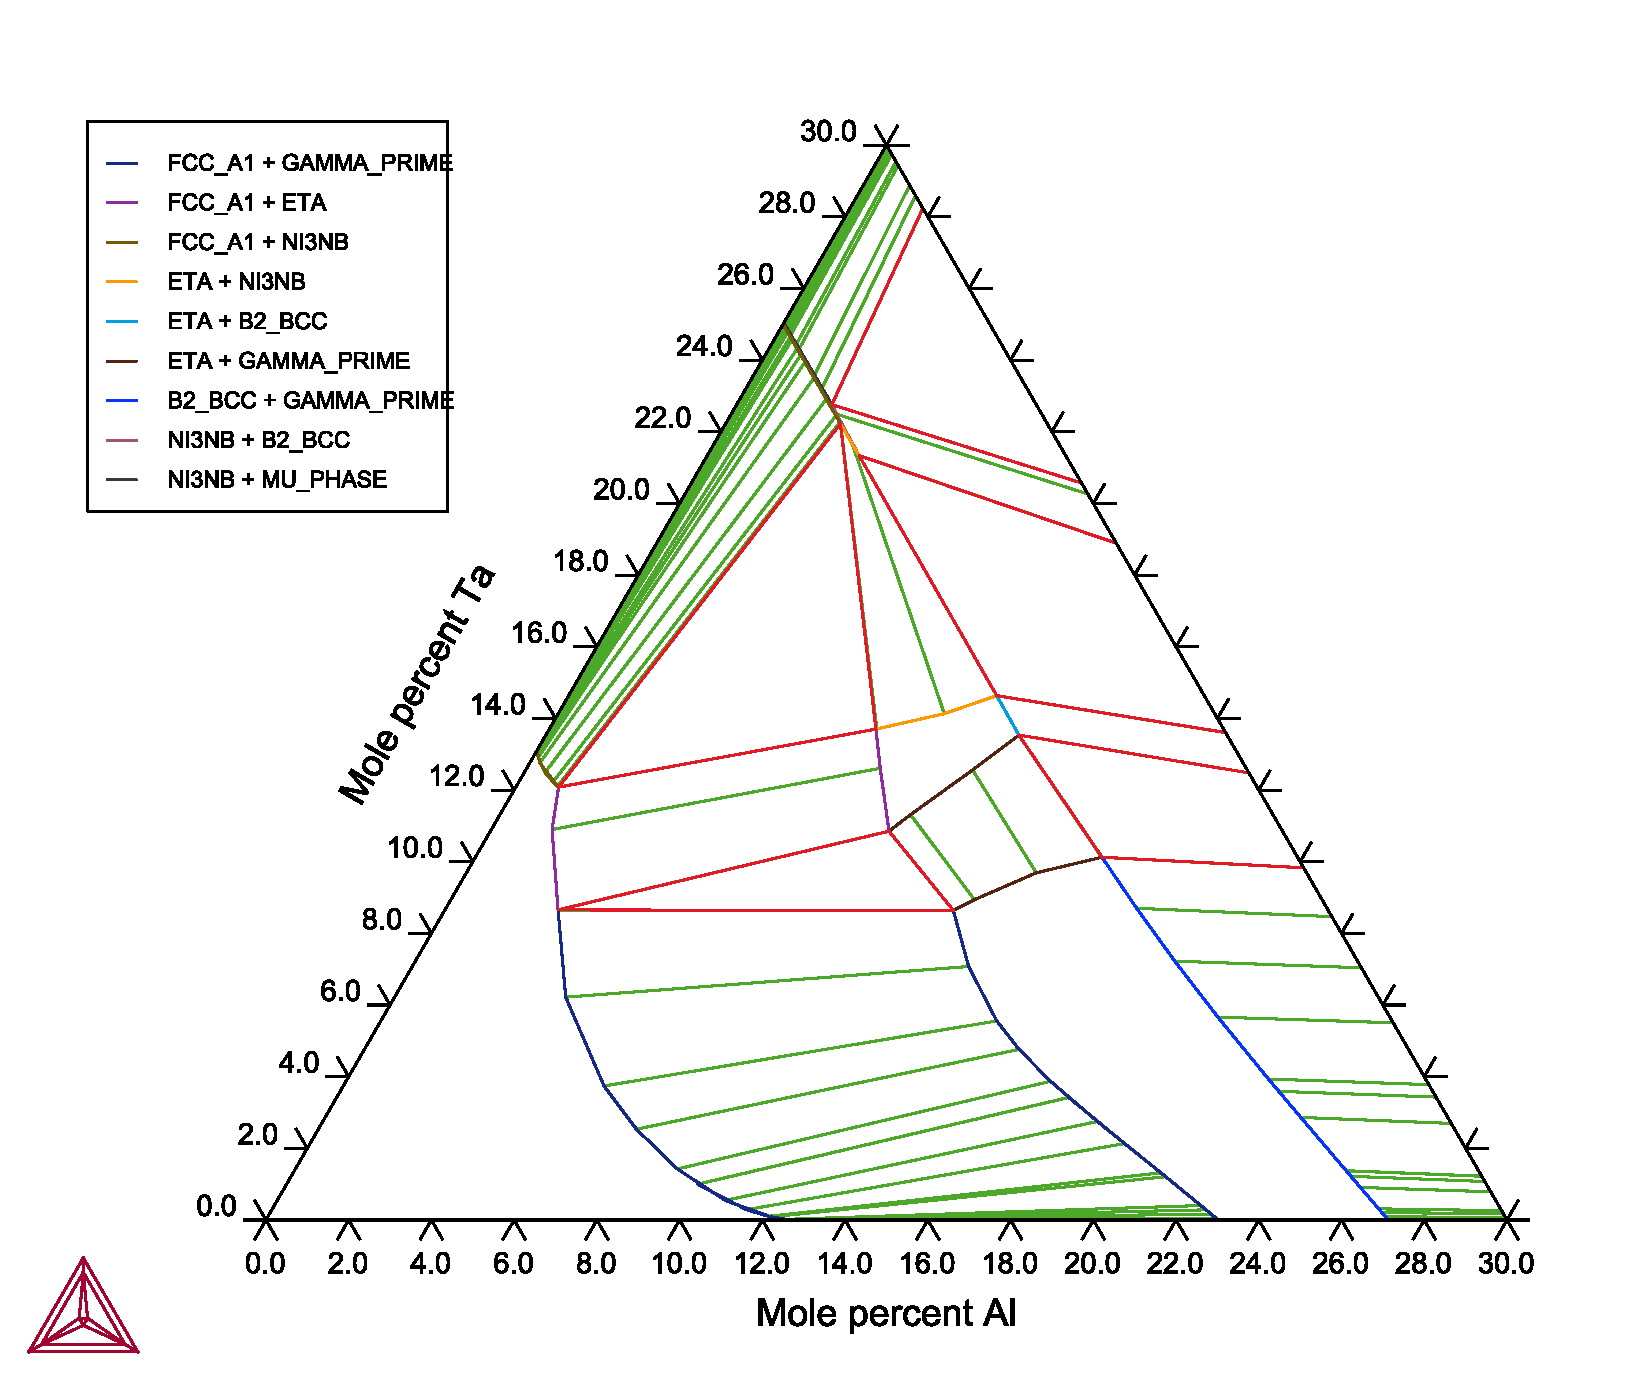
\includegraphics[width=0.5\textwidth]{graficas/Q2_NiAlTa_ternary_800C.pdf}
    }
  \subfloat[900°C\label{fig:900C}]{
    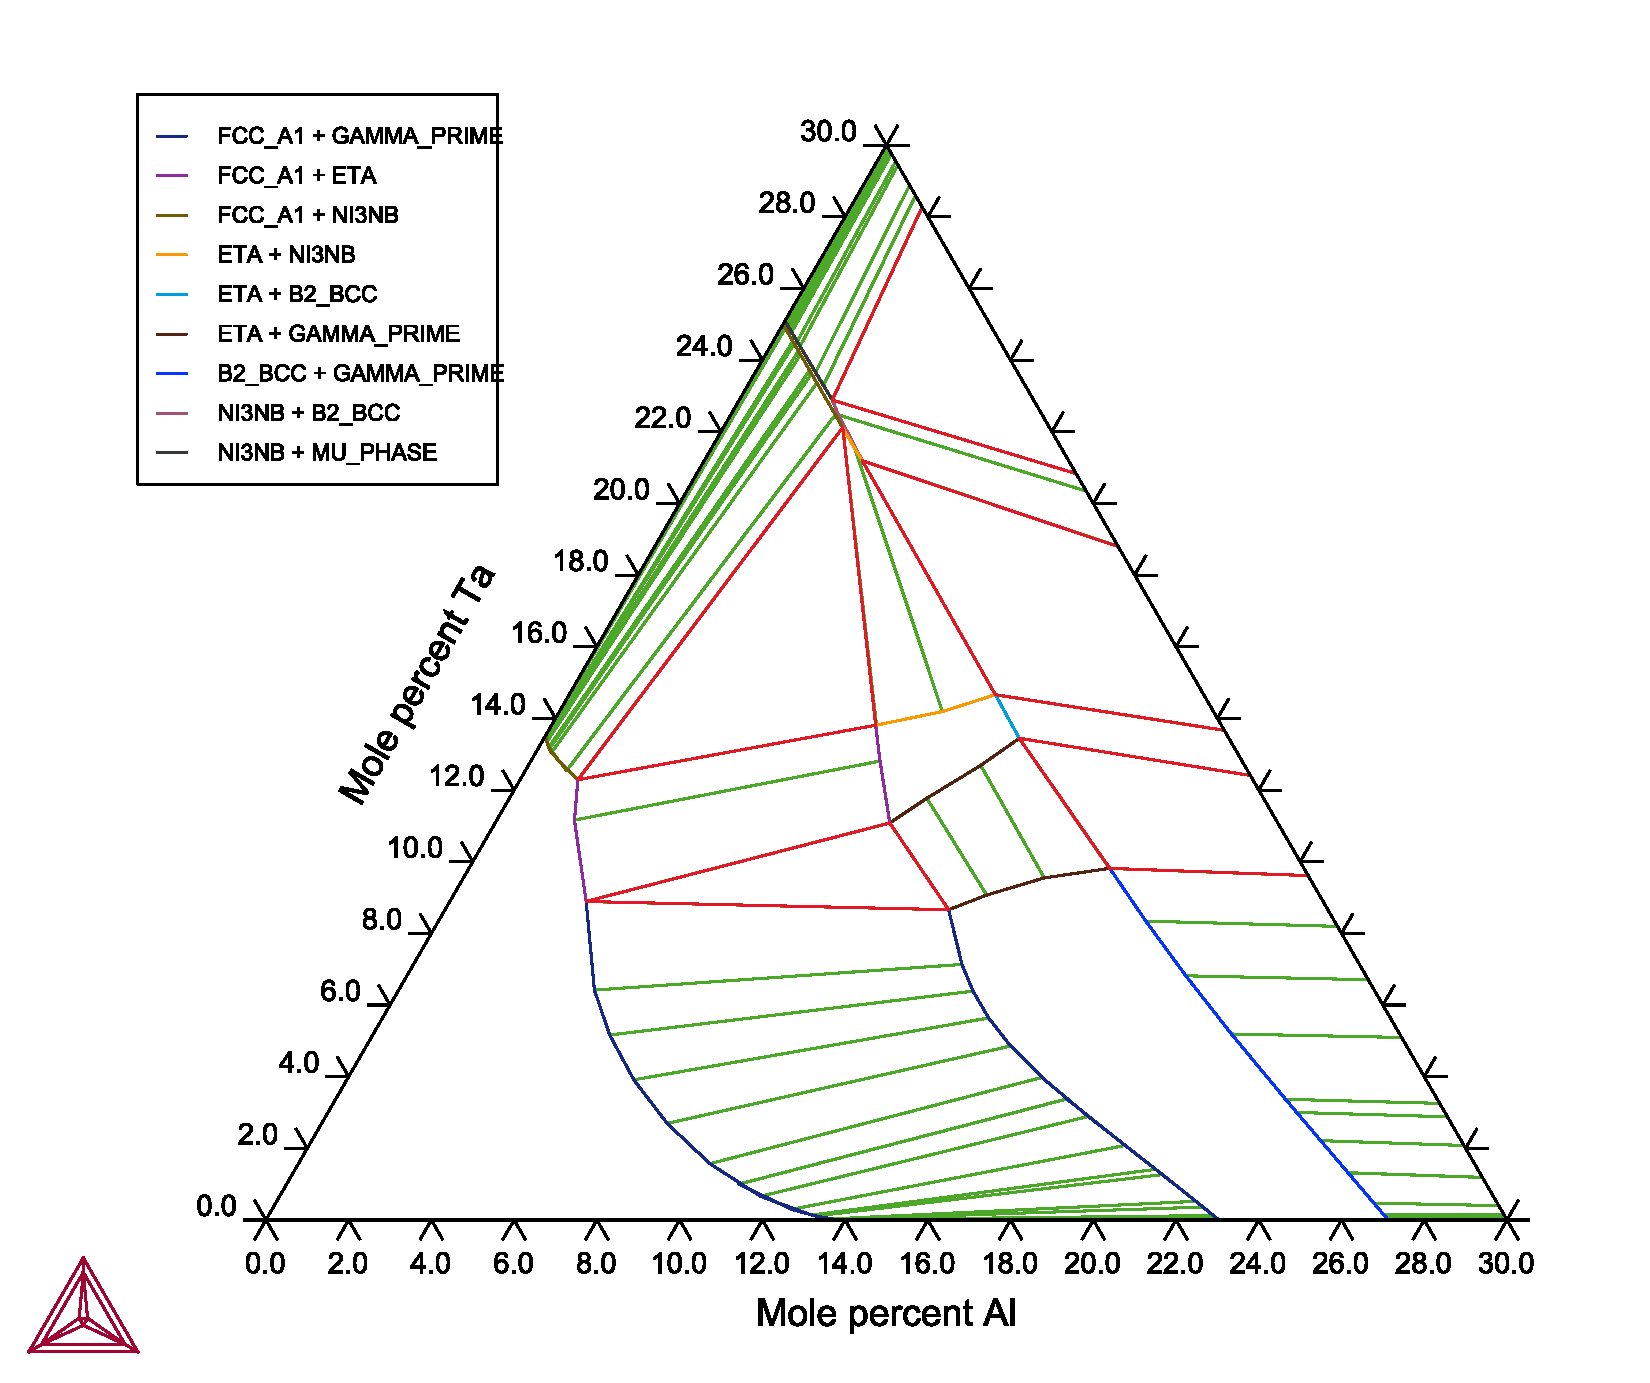
\includegraphics[width=0.5\textwidth]{graficas/Q2_NiAlTa_ternary_900C.pdf}
    }
  \caption{\centering Ni-Al-Ta ternary diagram at different temperatures \\
  \textit{Source: diagrams generated with ThermoCalc \citep{thermocalc}.}}
  \label{fig:diagram02}
\end{figure}

As temperature increases, the increase on the $\gamma$ phase is more evident, where the bondary line of the $\gamma$ phase moves from approximately $15\%$ at $10000$°C, in figure \ref{fig:1000C}, to $16\%$ at $1100$°C, in figure \ref{fig:1100C}. The change is more evident as the temperature increases to $1200$°C and $1300$°C, as it is shown in figures \ref{fig:1200C} and \ref{fig:1300C}; where at a temperature of $1200$°C the boundary can be found at $18\%$ and when the temperature is increased to $1300$°C the boundary is at $20\%$.

\begin{figure}[H]
  \centering
  \ContinuedFloat
  \subfloat[1000°C\label{fig:1000C}]{
    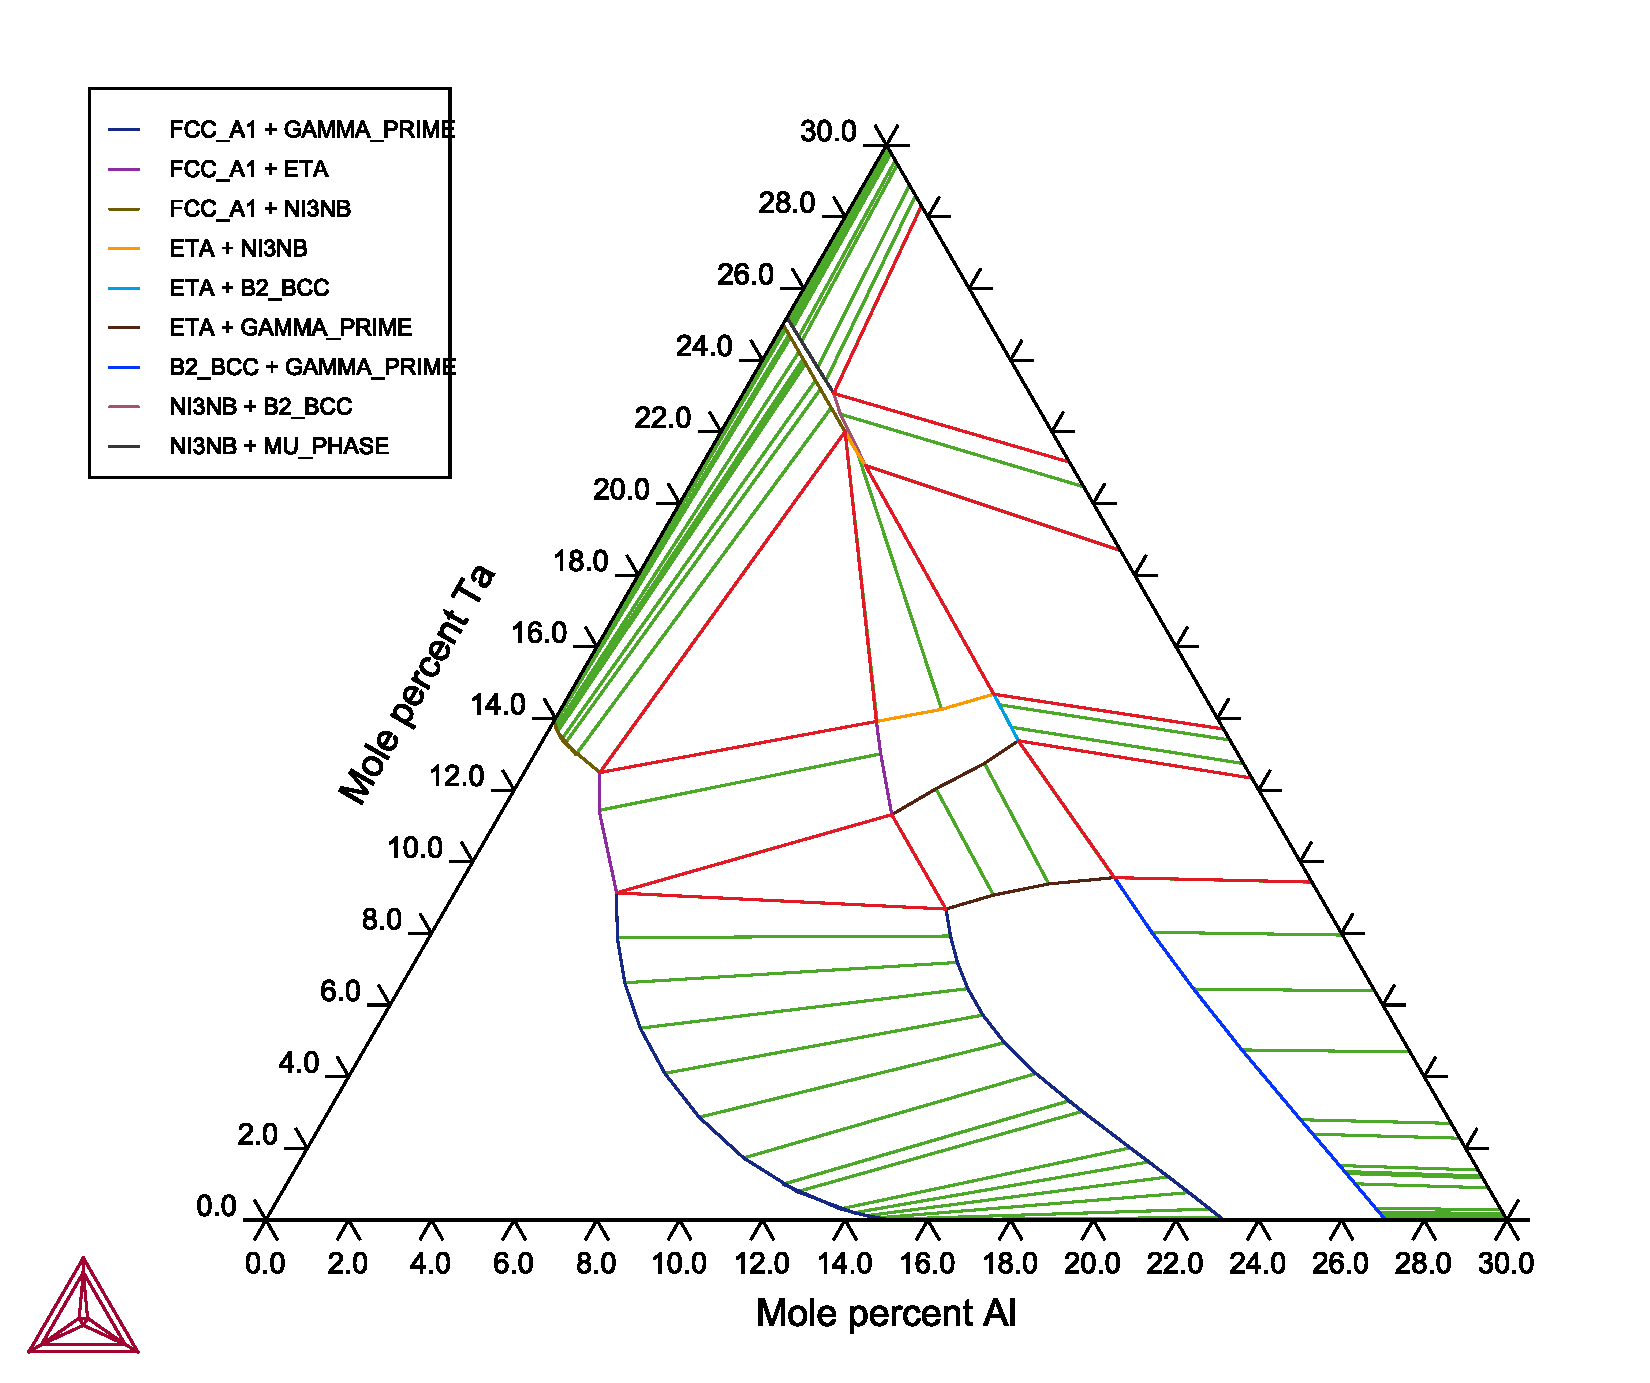
\includegraphics[width=0.5\textwidth]{graficas/Q2_NiAlTa_ternary_1000C.pdf}
    }
  \subfloat[1100°C\label{fig:1100C}]{
    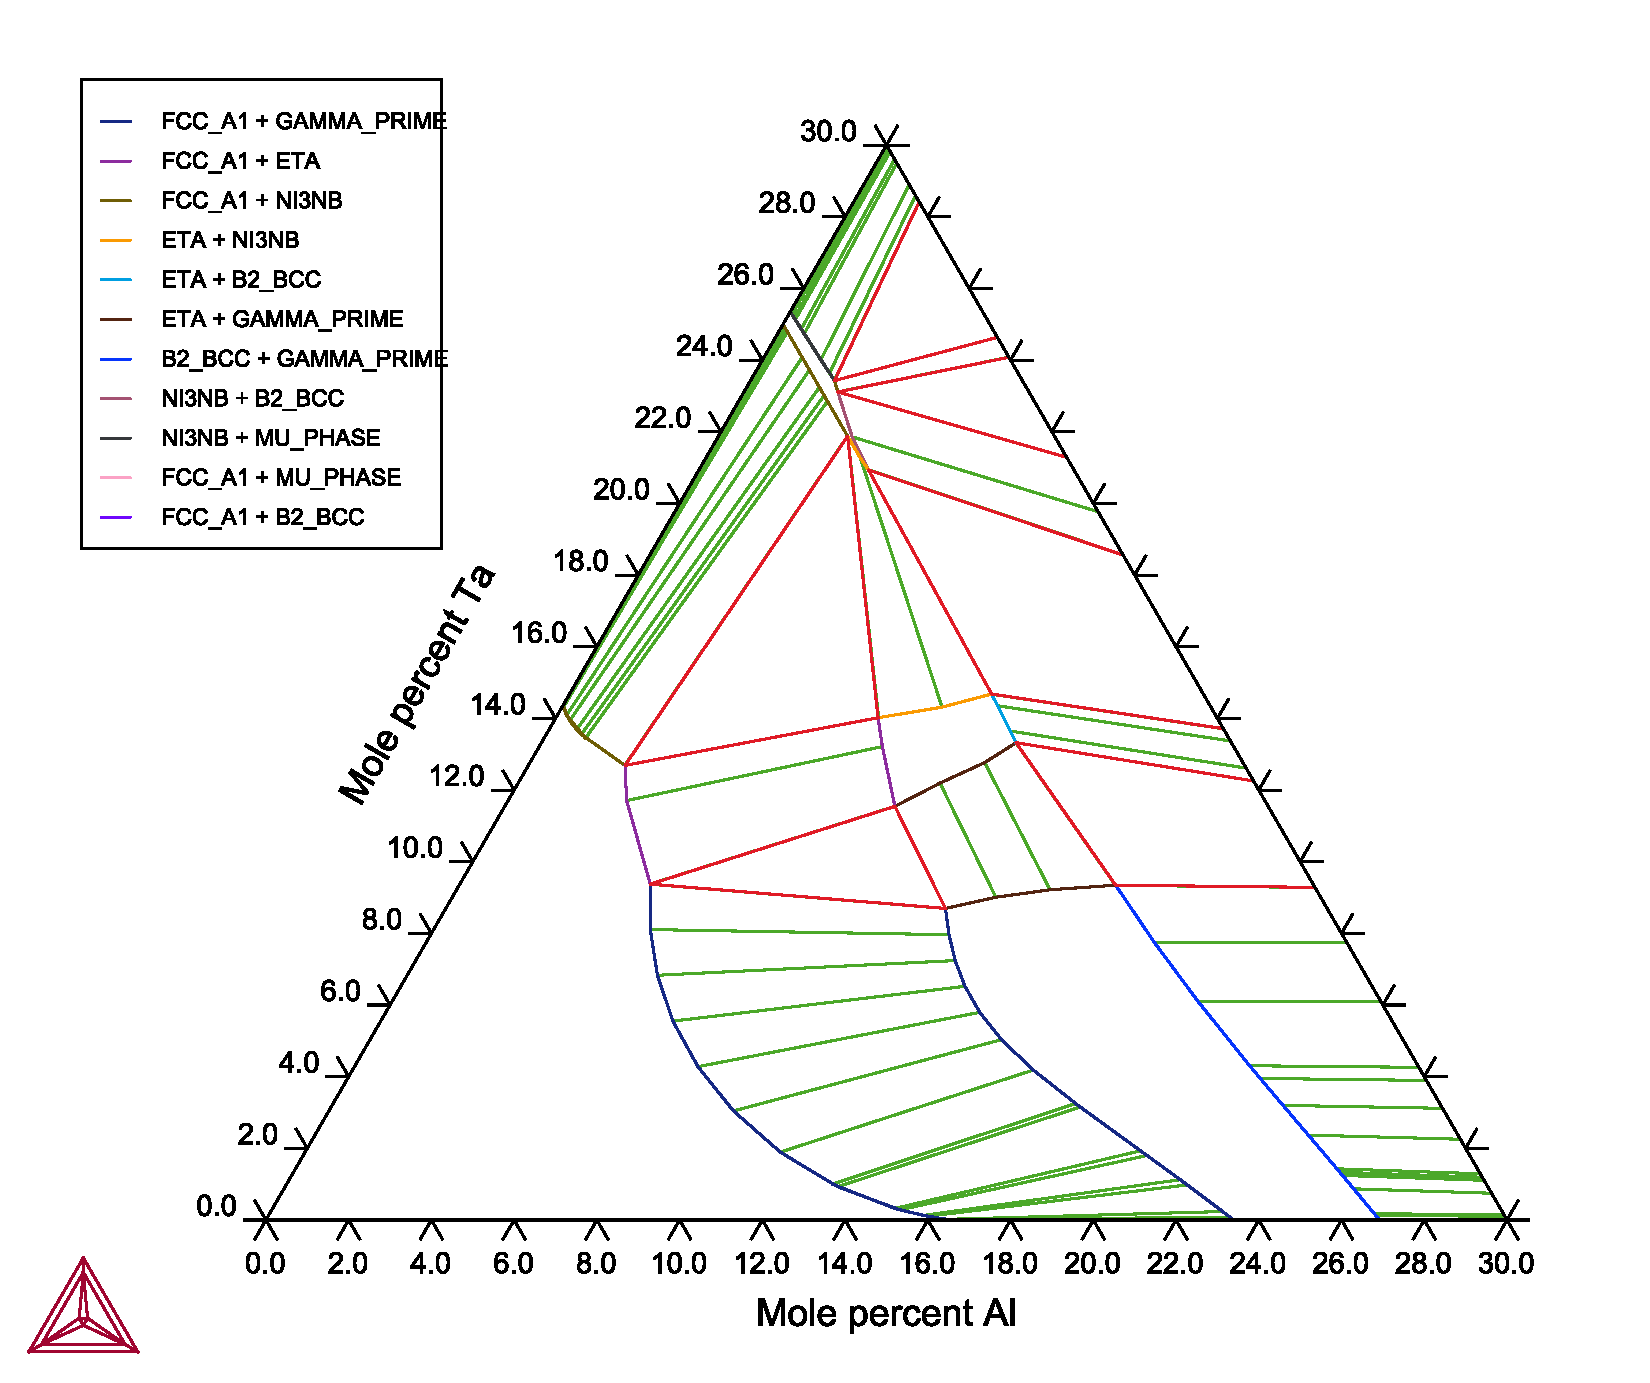
\includegraphics[width=0.5\textwidth]{graficas/Q2_NiAlTa_ternary_1100C.pdf}
    } \\
  \subfloat[1200°C\label{fig:1200C}]{
    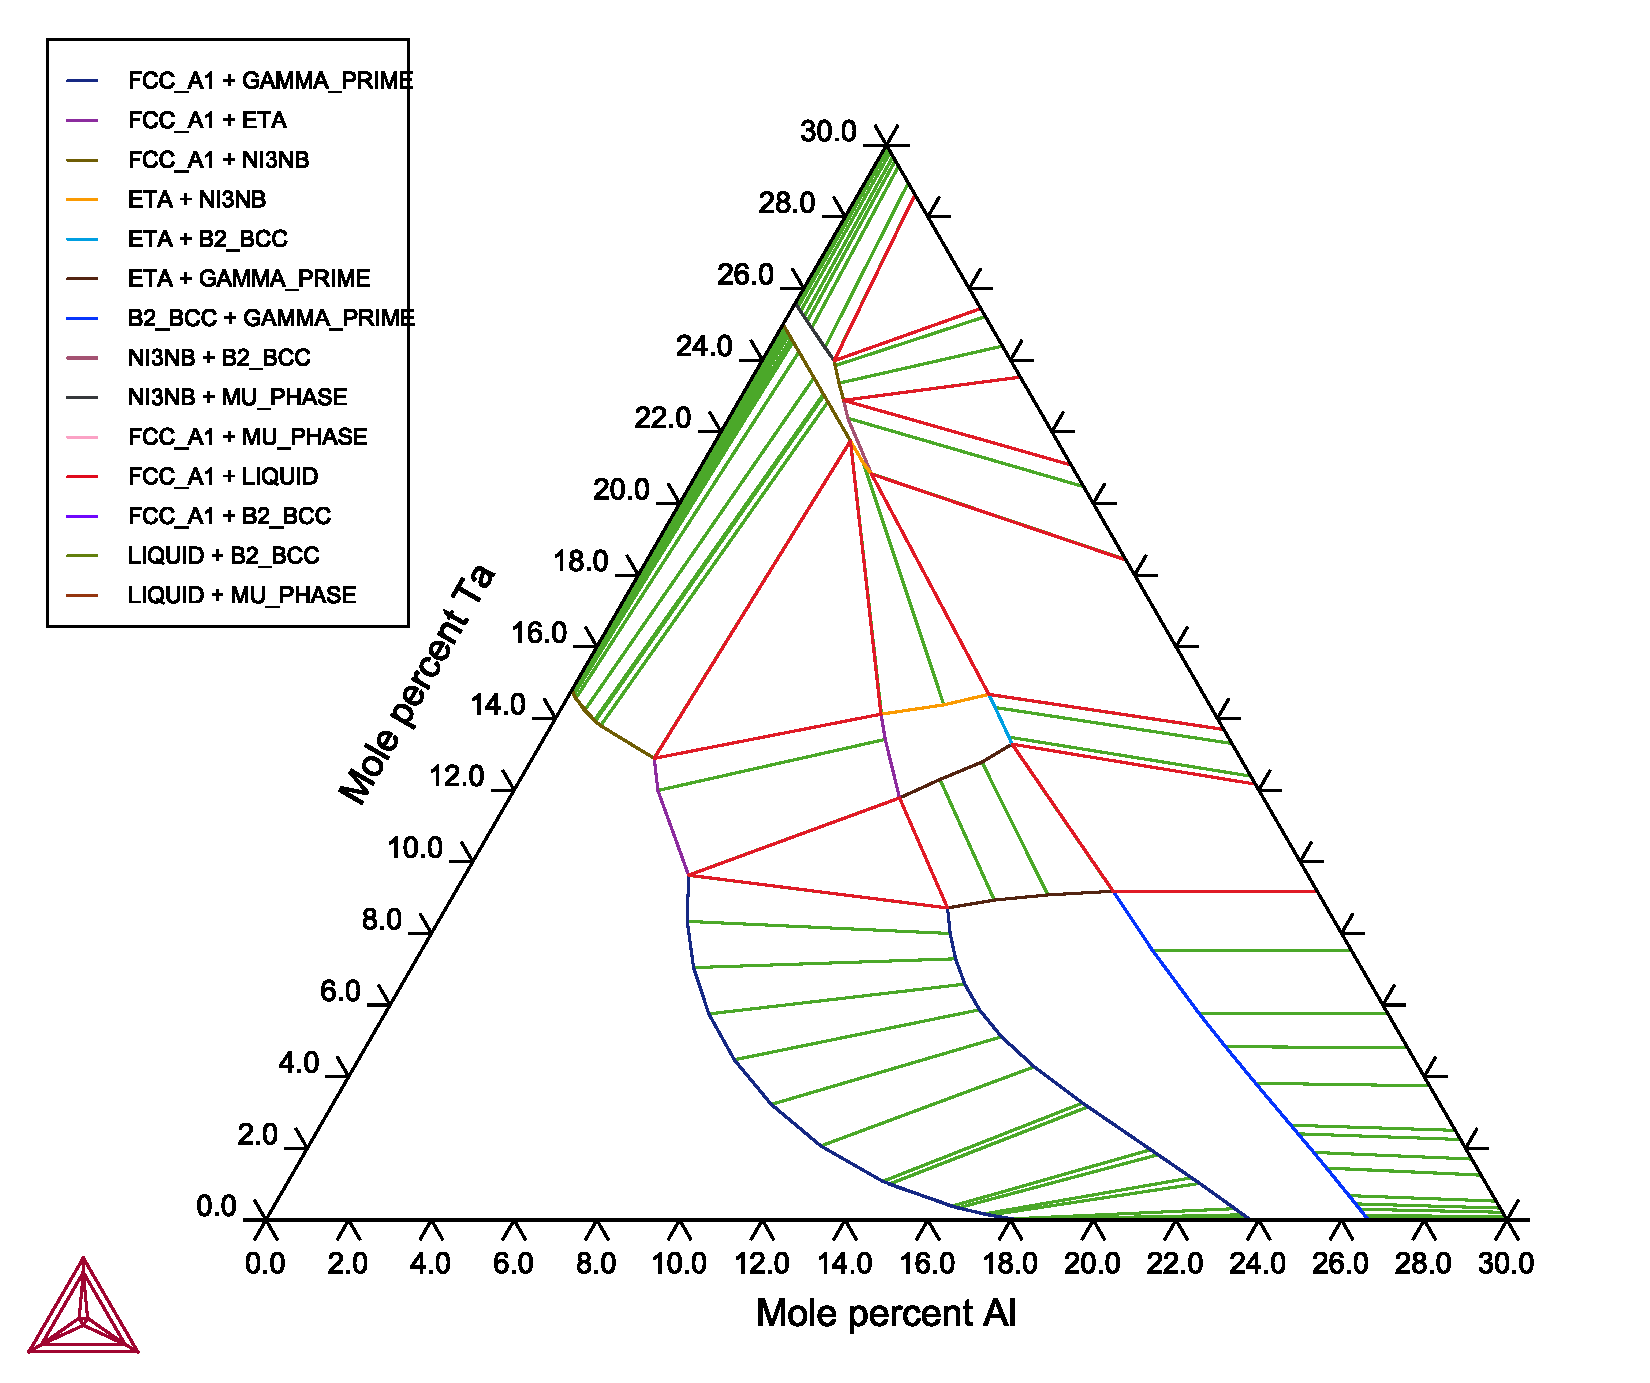
\includegraphics[width=0.5\textwidth]{graficas/Q2_NiAlTa_ternary_1200C.pdf}
    }
  \subfloat[1300°C\label{fig:1300C}]{
    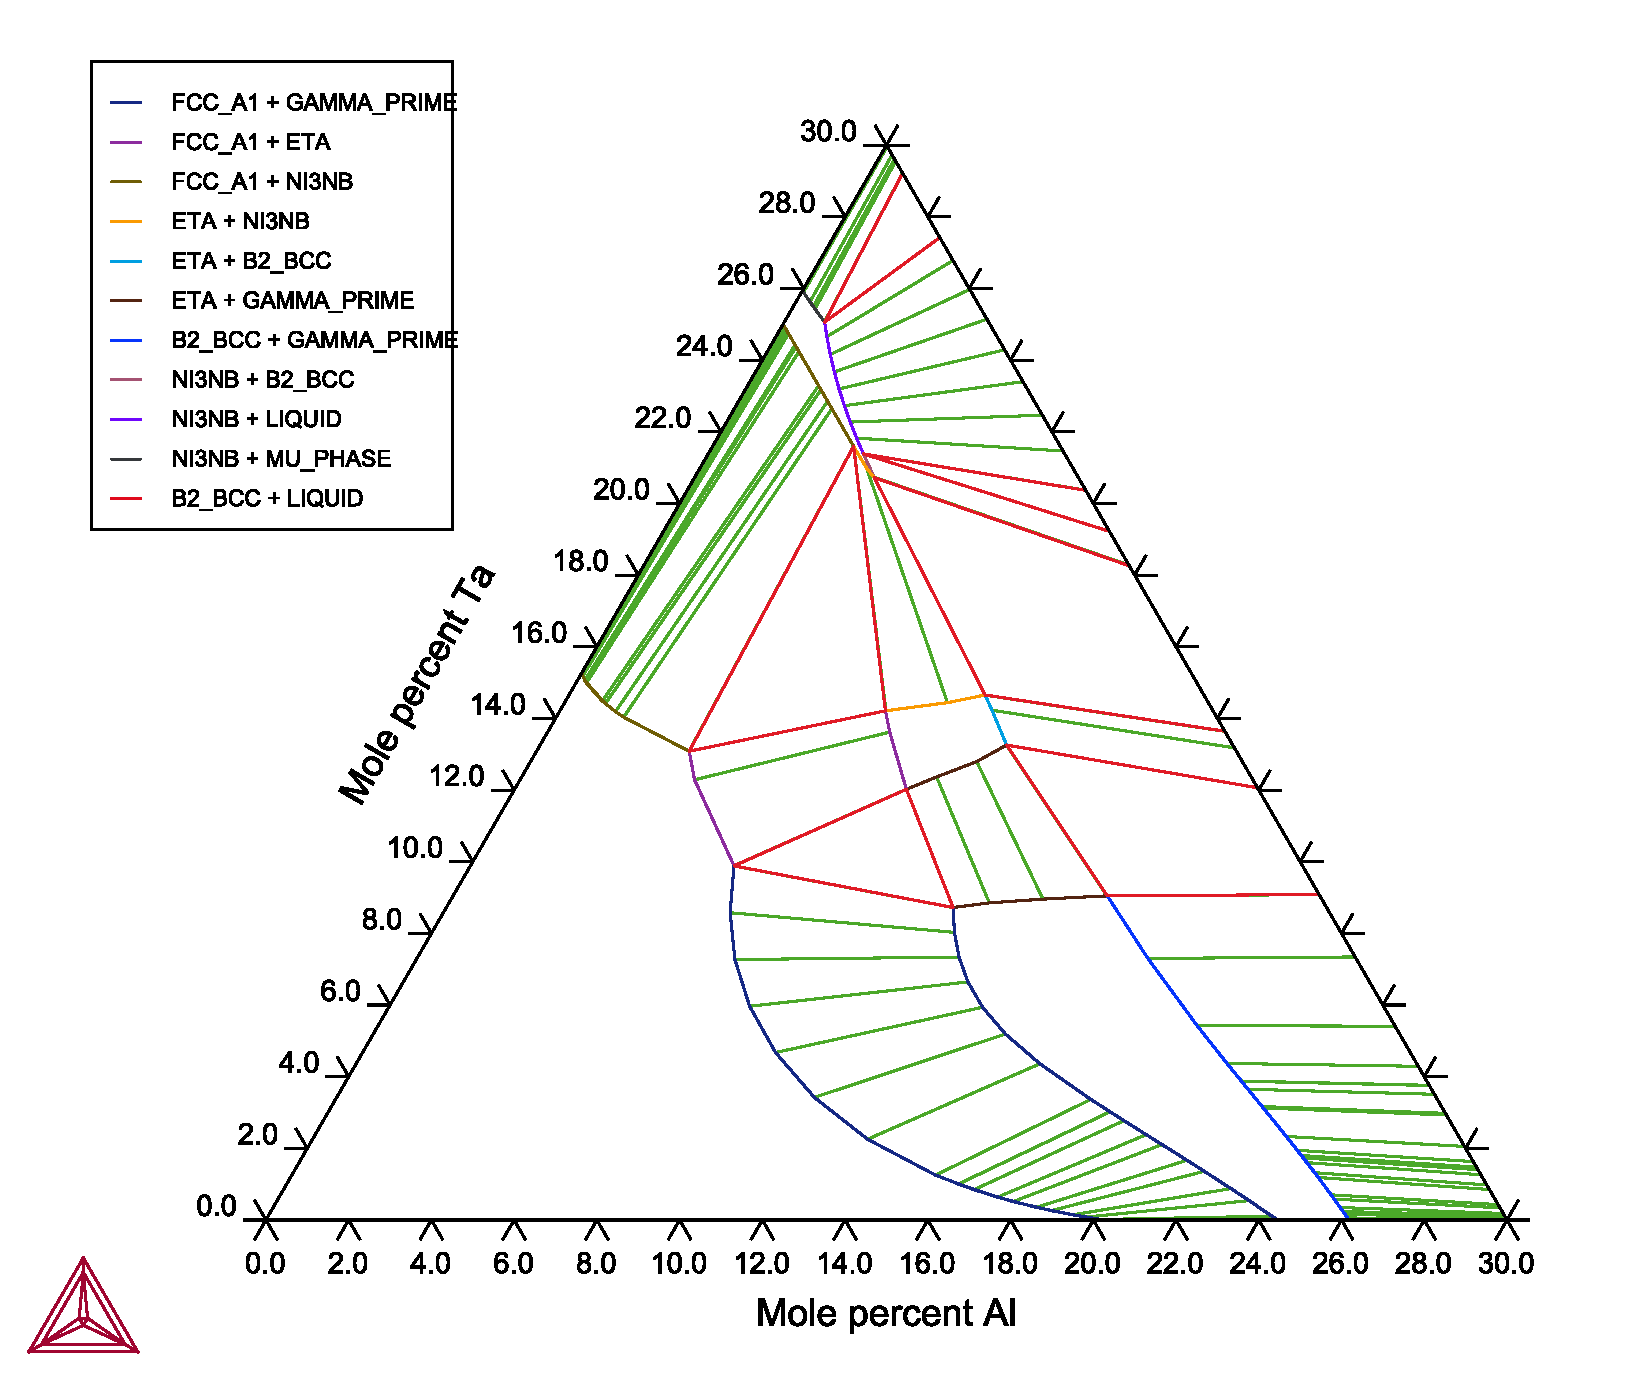
\includegraphics[width=0.5\textwidth]{graficas/Q2_NiAlTa_ternary_1300C.pdf}
    }
  \caption[]{\centering Ni-Al-Ta ternary diagram at different temperatures \\
  \textit{Source: diagrams generated with ThermoCalc \citep{thermocalc}.}}
\end{figure}

Along with the increase of the area that is occupied by the $\gamma$ phase, there is also a decrease on the area of the $\gamma'$ phase. These changes can indicate that there is a dependence on temperature on the equilibrium of the $\gamma$ and $\gamma'$ phases in the Ni-Al-Ta alloy.


\newpage
\subsection{Ni-Al-Ta alloys for which $\gamma'$ phase fraction is optimal}

The optimal fraction is that for which $\gamma'$ is $75\%$. To find the optimal fractions for $\gamma'$ the calculation tool \textit{One axis} was used, the results obtained are presented in table \ref{tab:tab02}:

\begin{table}[h]
  \centering
    \begin{tabular}{rrr}
        \multicolumn{1}{c}{\textbf{Mole $\%$ Ni}} & \multicolumn{1}{c}{\textbf{Mole $\%$ Al}} & \multicolumn{1}{c}{\textbf{Mole $\%$ Ta}} \\ \hline \hline
        78.8510 & 21.1490 & 7.6838e-10 \\
        79.5936 & 19.4064 & 1 \\
        80.3959 & 17.6041 & 2 \\
        81.1163 & 15.8837 & 3 \\
        81.6316 & 14.3684 & 4 \\
        81.9001 & 13.0999 & 5 \\
        81.9378 & 12.0622 & 6 \\
        81.7829 & 11.2171 & 7 \\
        81.4782 & 10.5218 & 8 \\
        81.1562 & 10.0517 & 8.7921
    \end{tabular}
  \caption{\centering Molar fractions of the Ni-Al-Ta alloy for which the $\gamma'$ phase fraction is optimal.\\
  \textit{Source: Calculations obtained using ThermoCalc \citep{thermocalc}}}
  \label{tab:tab02}
\end{table}

The fractions of Ni, Al and Ta for which the $\gamma'$ fraction is optimal presented in table \ref{tab:tab02} were plotted ternary phase diagram, figure \ref{fig:diagram03}.

\begin{figure}[h]
  \centering
  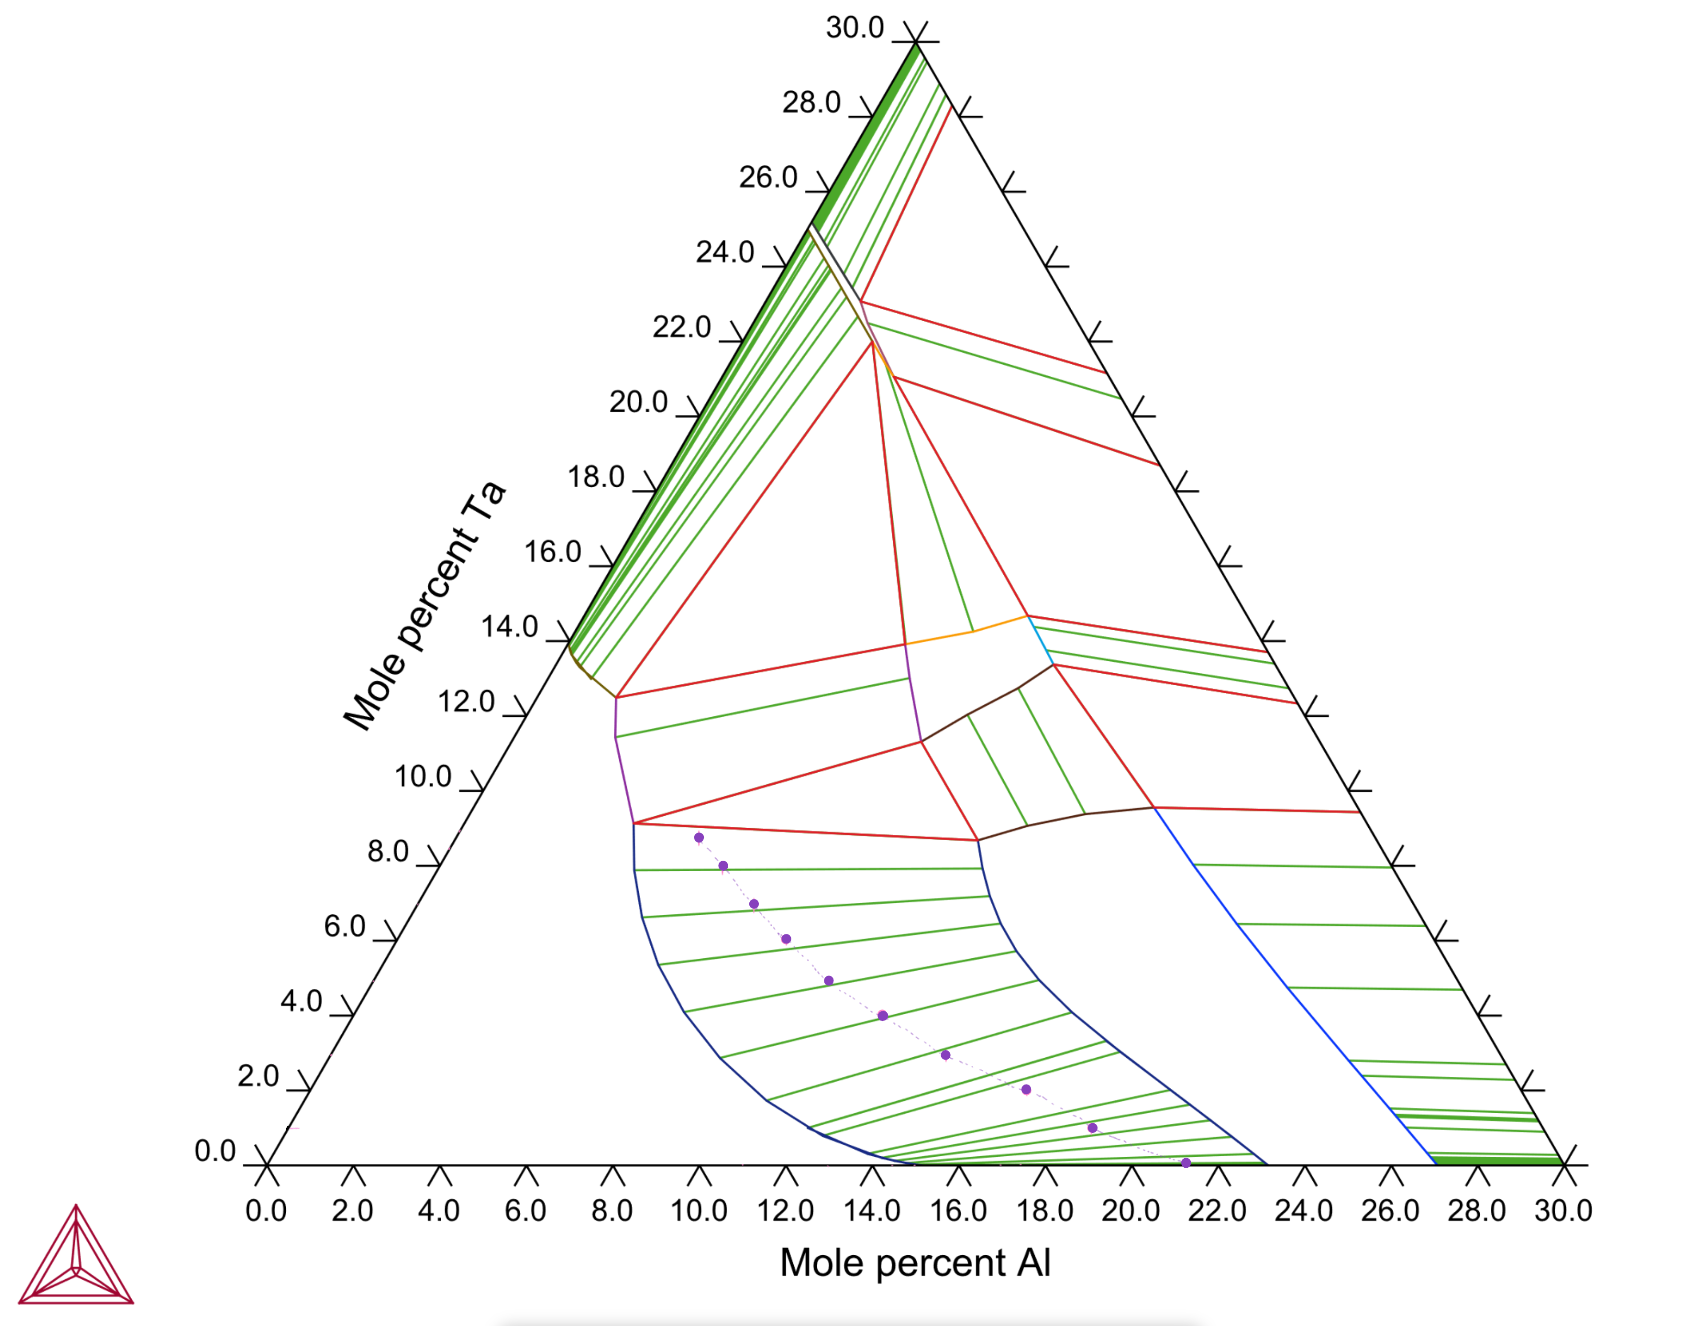
\includegraphics[width=0.95\textwidth]{graficas/Q2_NiAlTa_ternary03.png}
  \caption{\centering Ni-Al-Ta ternary phase diagram with compositions for optimal $\gamma'$ phase fraction. \\
  \textit{Diagram generated using \textit{ThermoCalc} \citep{thermocalc}, phase compositions plotted by the author.}}
  \label{fig:diagram03}
\end{figure}
\clearpage
\section{}

\subsection{Show that the alloys chosen are not ideal}

Lattice parameters:
\begin{align}
    \begin{split}
        a_\gamma &= 3.523 + 0.179 Al + 0.700Ta + 0.110 Cr + 0.444W+ 0.441 Re \\
        & + 0.478Mo + 0.096 Co \\
        a_{\gamma'} &= 3.558 + 0.500Ta ¡ 0.004 Cr + 0.194W+ 0.262 Re + 0.208Mo
    \end{split}
\end{align}

Lattice misfit equation
\begin{align}
    \delta &= 2\times\left[\dfrac{a_{\gamma'}-a_\gamma}{a_{\gamma'}+a_\gamma}\right]
\end{align}

\begin{table}[h]
    \centering
    \begin{tabular}{rrrrrrrrr}
        \multicolumn{1}{c}{Ni$_\gamma$} & \multicolumn{1}{c}{Al$_\gamma$} & \multicolumn{1}{c}{Ta$_\gamma$} & \multicolumn{1}{c}{Ni$_{\gamma'}$} & \multicolumn{1}{c}{Al$_{\gamma'}$} & \multicolumn{1}{c}{Ta$_{\gamma'}$} & \multicolumn{1}{c}{$a_\gamma$} & \multicolumn{1}{c}{$a_{\gamma'}$} & \multicolumn{1}{c}{$\delta$} \\ \hline \hline
        0.8633 & 0.1317 & 0.0050 & 0.7842 & 0.1908 & 0.0250 & 3.5501 & 3.5705 & 0.0057 \\0.8721 & 0.1156 & 0.0123 & 0.7909 & 0.1732 & 0.0359 & 3.5523 & 3.5760 & 0.0066 \\0.8789 & 0.0979 & 0.0232 & 0.7954 & 0.1590 & 0.0456 & 3.5568 & 3.5808 & 0.0067 \\0.8826 & 0.0809 & 0.0365 & 0.7978 & 0.1477 & 0.0545 & 3.5630 & 3.5853 & 0.0062 \\0.8830 & 0.0661 & 0.0509 & 0.7982 & 0.1388 & 0.0630 & 3.5705 & 3.5895 & 0.0053 \\0.8803 & 0.0541 & 0.0655 & 0.7970 & 0.1315 & 0.0715 & 3.5786 & 3.5937 & 0.0042 \\0.8751 & 0.0448 & 0.0800 & 0.7947 & 0.1253 & 0.0800 & 3.5870 & 3.5980 & 0.0030 \\0.8696 & 0.0391 & 0.0913 & 0.7922 & 0.1210 & 0.0868 & 3.5939 & 3.6014 & 0.0021 \\0.8696 & 0.0391 & 0.0913 & 0.7922 & 0.1210 & 0.0868 & 3.5939 & 3.6014 & 0.0021 \\0.8696 & 0.0391 & 0.0913 & 0.7922 & 0.1210 & 0.0868 & 3.5939 & 3.6014 & 0.0021 \\0.8696 & 0.0391 & 0.0913 & 0.7922 & 0.1210 & 0.0868 & 3.5939 & 3.6014 & 0.0021 \\0.8696 & 0.0391 & 0.0913 & 0.7922 & 0.1210 & 0.0868 & 3.5939 & 3.6014 & 0.0021 \\0.8633 & 0.1317 & 0.0050 & 0.7842 & 0.1908 & 0.0250 & 3.5501 & 3.5705 & 0.0057 \\0.8547 & 0.1439 & 0.0013 & 0.7763 & 0.2108 & 0.0129 & 3.5497 & 3.5644 & 0.0041 \\0.8485 & 0.1515 & 0.0000 & 0.7685 & 0.2315 & 0.0000 & 3.5501 & 3.5580 & 0.0022
    \end{tabular}
    \caption{Lattice misfit, $\delta$, calculated for the Ni-Al-Ta alloy using the compositions (molar fractions) of the elements present in $\gamma$ and $\gamma'$ phases obtained using\textit{ThermoCalc} \citep{thermocalc}. The calculations of $a_\gamma$, $a_{\gamma´}$ and $\delta$ were performed in Python \citep{mygit}}
    \label{tab:tab03}
\end{table}

From table \ref{tab:tab03} it can be seen that the values of $\delta$ are not equal to zero, which can indicate that the alloy is not ideal for the different compositions.

\newpage
\subsection{With additions of Cr, W, Re, Mo or mixture, find alloy for which the lattice misfit is close to zero}

The values of the lattice misfit for both $\gamma$ and $\gamma'$ phases were calculated using the molar fractions of the $\gamma$ and $\gamma'$ phases of different alloys of Ni-Al-Ta-X, where X is Cr, Mo, Re and W, obtained from a \textit{ThermoCalc} calculations. The results obtained are presented in tables \ref{tab:tab04}, ,\ref{tab:tab05}, \ref{tab:tab06} and \ref{tab:tab07} in the Appendix \ref{appendix}.

From the values of lattice misfit obtained for each alloy, the minimum value was extracted in order to know which composition gives a lattice misfit closer to zero, the results are presented in table \ref{tab:tab08}:

\begin{table}[H]
  \centering
  \begin{tabular}{rrrrrrrrrrr}
    \multicolumn{1}{c}{Ni$_\gamma$} & \multicolumn{1}{c}{Al$_\gamma$} & \multicolumn{1}{c}{Ta$_\gamma$} & \multicolumn{1}{c}{Cr$_\gamma$} & \multicolumn{1}{c}{Ni$_{\gamma'}$} & \multicolumn{1}{c}{Al$_{\gamma'}$} & \multicolumn{1}{c}{Ta$_{\gamma'}$} & \multicolumn{1}{c}{Cr$_{\gamma'}$} & \multicolumn{1}{c}{a$_\gamma$} & \multicolumn{1}{c}{a$_{\gamma'}$} & \multicolumn{1}{c}{$\delta$} \\ \hline \hline
    0.7434 & 0.0862 & 0.0077 & 0.1627 & 0.7528 & 0.1741 & 0.0347 & 0.0384 & 3.5617 & 3.5752 & 0.0038 \\\\
   \multicolumn{1}{c}{Ni$_\gamma$} & \multicolumn{1}{c}{Al$_\gamma$} & \multicolumn{1}{c}{Ta$_\gamma$} & \multicolumn{1}{c}{Mo$_\gamma$} & \multicolumn{1}{c}{Ni$_{\gamma'}$} & \multicolumn{1}{c}{Al$_{\gamma'}$} & \multicolumn{1}{c}{Ta$_{\gamma'}$} & \multicolumn{1}{c}{Mo$_{\gamma'}$} & \multicolumn{1}{c}{$a_\gamma$} & \multicolumn{1}{c}{$a_{\gamma'}$} & \multicolumn{1}{c}{$\delta$} \\ \hline \hline
   0.8430 & 0.0843 & 0.0196 & 0.0530 & 0.7731 & 0.1641 & 0.0307 & 0.0320 & 3.5772 & 3.5734 & 0.0011 \\\\
   \multicolumn{1}{c}{Ni$_\gamma$} & \multicolumn{1}{c}{Al$_\gamma$} & \multicolumn{1}{c}{Ta$_\gamma$} & \multicolumn{1}{c}{Re$_\gamma$} & \multicolumn{1}{c}{Ni$_{\gamma'}$} & \multicolumn{1}{c}{Al$_{\gamma'}$} & \multicolumn{1}{c}{Ta$_{\gamma'}$} & \multicolumn{1}{c}{Re$_{\gamma'}$} & \multicolumn{1}{c}{a$_\gamma$} & \multicolumn{1}{c}{a$_{\gamma'}$} & \multicolumn{1}{c}{$\delta$} \\ \hline \hline
   0.8303 & 0.1157 & 0.0087 & 0.0453 & 0.7790 & 0.1798 & 0.0340 & 0.0072 & 3.5698 & 3.5769 & 0.0020 \\\\
   \multicolumn{1}{c}{Ni$_\gamma$} & \multicolumn{1}{c}{Al$_\gamma$} & \multicolumn{1}{c}{Ta$_\gamma$} & \multicolumn{1}{c}{W$_\gamma$} & \multicolumn{1}{c}{Ni$_{\gamma'}$} & \multicolumn{1}{c}{Al$_{\gamma'}$} & \multicolumn{1}{c}{Ta$_{\gamma'}$} & \multicolumn{1}{c}{W$_{\gamma'}$} & \multicolumn{1}{c}{a$_\gamma$} & \multicolumn{1}{c}{a$_{\gamma'}$} & \multicolumn{1}{c}{$\delta$} \\ \hline \hline
   0.8711 & 0.0797 & 0.0199 & 0.0293 & 0.7871 & 0.1588 & 0.0300 & 0.0241 & 3.5642 & 3.5777 & 0.0038
  \end{tabular}
  \caption{Minimum values of lattice misfit, $\delta$, for each alloy calculated using Python \citep{mygit}}
  \label{tab:tab08}
\end{table}

From the values presented in table \ref{tab:tab08}, the minimum value of all the alloys was extracted, which is shown in table \ref{tab:tab09}, with a misfit value of $0.0011$, being the closet value for all the alloys.

\begin{table}[h]
  \begin{tabular}{rrrrrrrrrrrrrrrrr}
    \multicolumn{1}{c}{Ni$_\gamma$} & \multicolumn{1}{c}{Al$_\gamma$} & \multicolumn{1}{c}{Ta$_\gamma$} & \multicolumn{1}{c}{Mo$_\gamma$} & \multicolumn{1}{c}{Ni$_{\gamma'}$} & \multicolumn{1}{c}{Al$_{\gamma'}$} & \multicolumn{1}{c}{Ta$_{\gamma'}$} & \multicolumn{1}{c}{Mo$_{\gamma'}$} & \multicolumn{1}{c}{$a_\gamma$} & \multicolumn{1}{c}{$a_{\gamma'}$} & \multicolumn{1}{c}{$\delta$} \\ \hline \hline
    0.8430 & 0.0843 & 0.0196 & 0.0530 & 0.7731 & 0.1641 & 0.0307 & 0.0320 & 3.5772 & 3.5734 & 0.0011
  \end{tabular}
  \caption{Minim value of lattice misfit from all alloys, corresponding to the Ni-Al-Ta-Mo alloy. Table generated using Python \citep{mygit}.}
  \label{tab:tab09}
\end{table}

\newpage
\subsection{Do Cr, W, Re and Mo alter significantly the fraction of $\gamma'$ present?}

Figure \ref{fig:diagram04} shows the graphs of the amount of all phases as a function of the mole percent of Cr, Mo, Re and W. The red line is the $\gamma'$ composition and as it can be seen in all four plots the behavior of the $\gamma'$ phase line is different with each system. From these plots it can be said that the presence of Cr, W, Re and Mo do have an effect ont he fraction of $\gamma'$ present.


\begin{figure}[H]
  \centering
  \subfloat[Cr\label{fig:cr}]{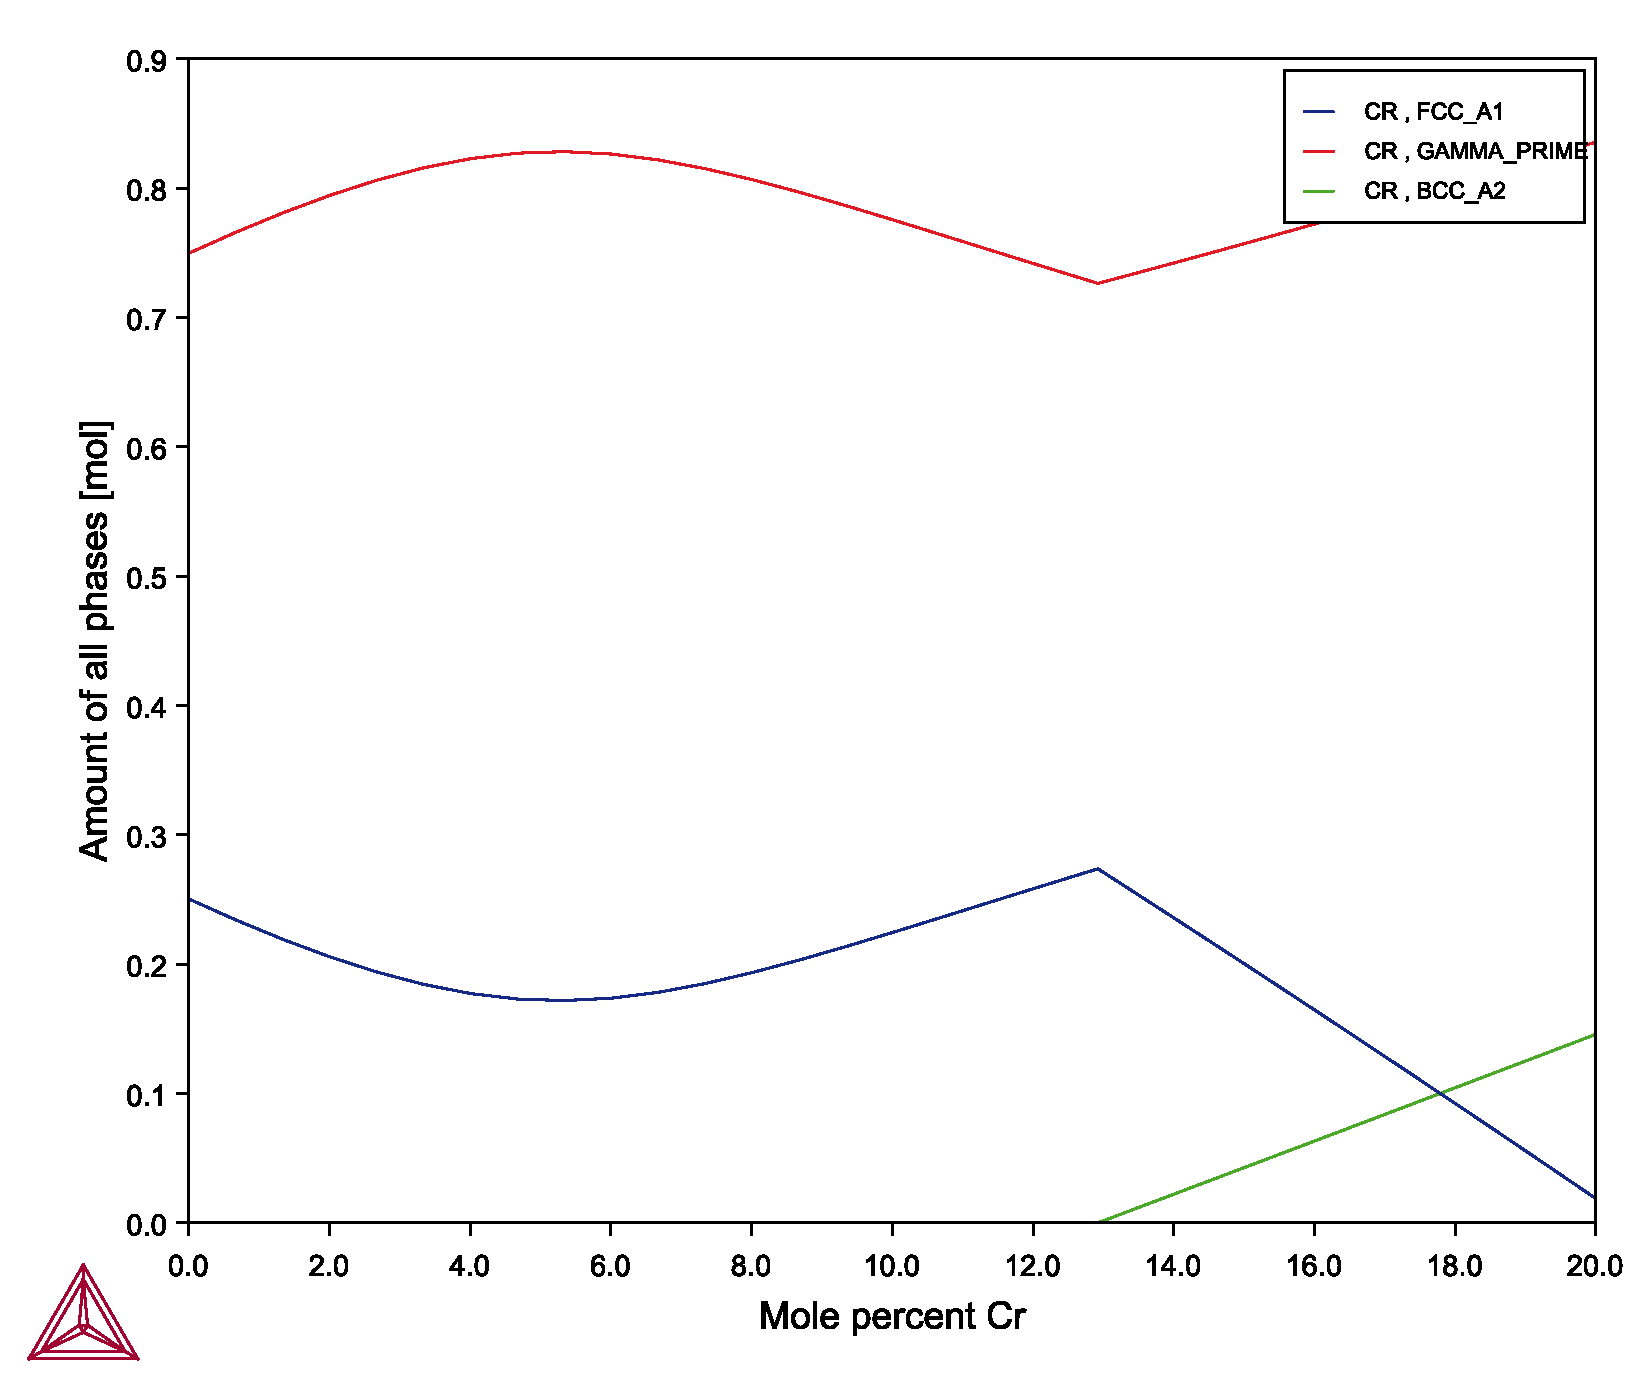
\includegraphics[width=0.5\textwidth]{graficas/Q3_Cr.pdf}}
  \subfloat[Mo\label{fig:mo}]{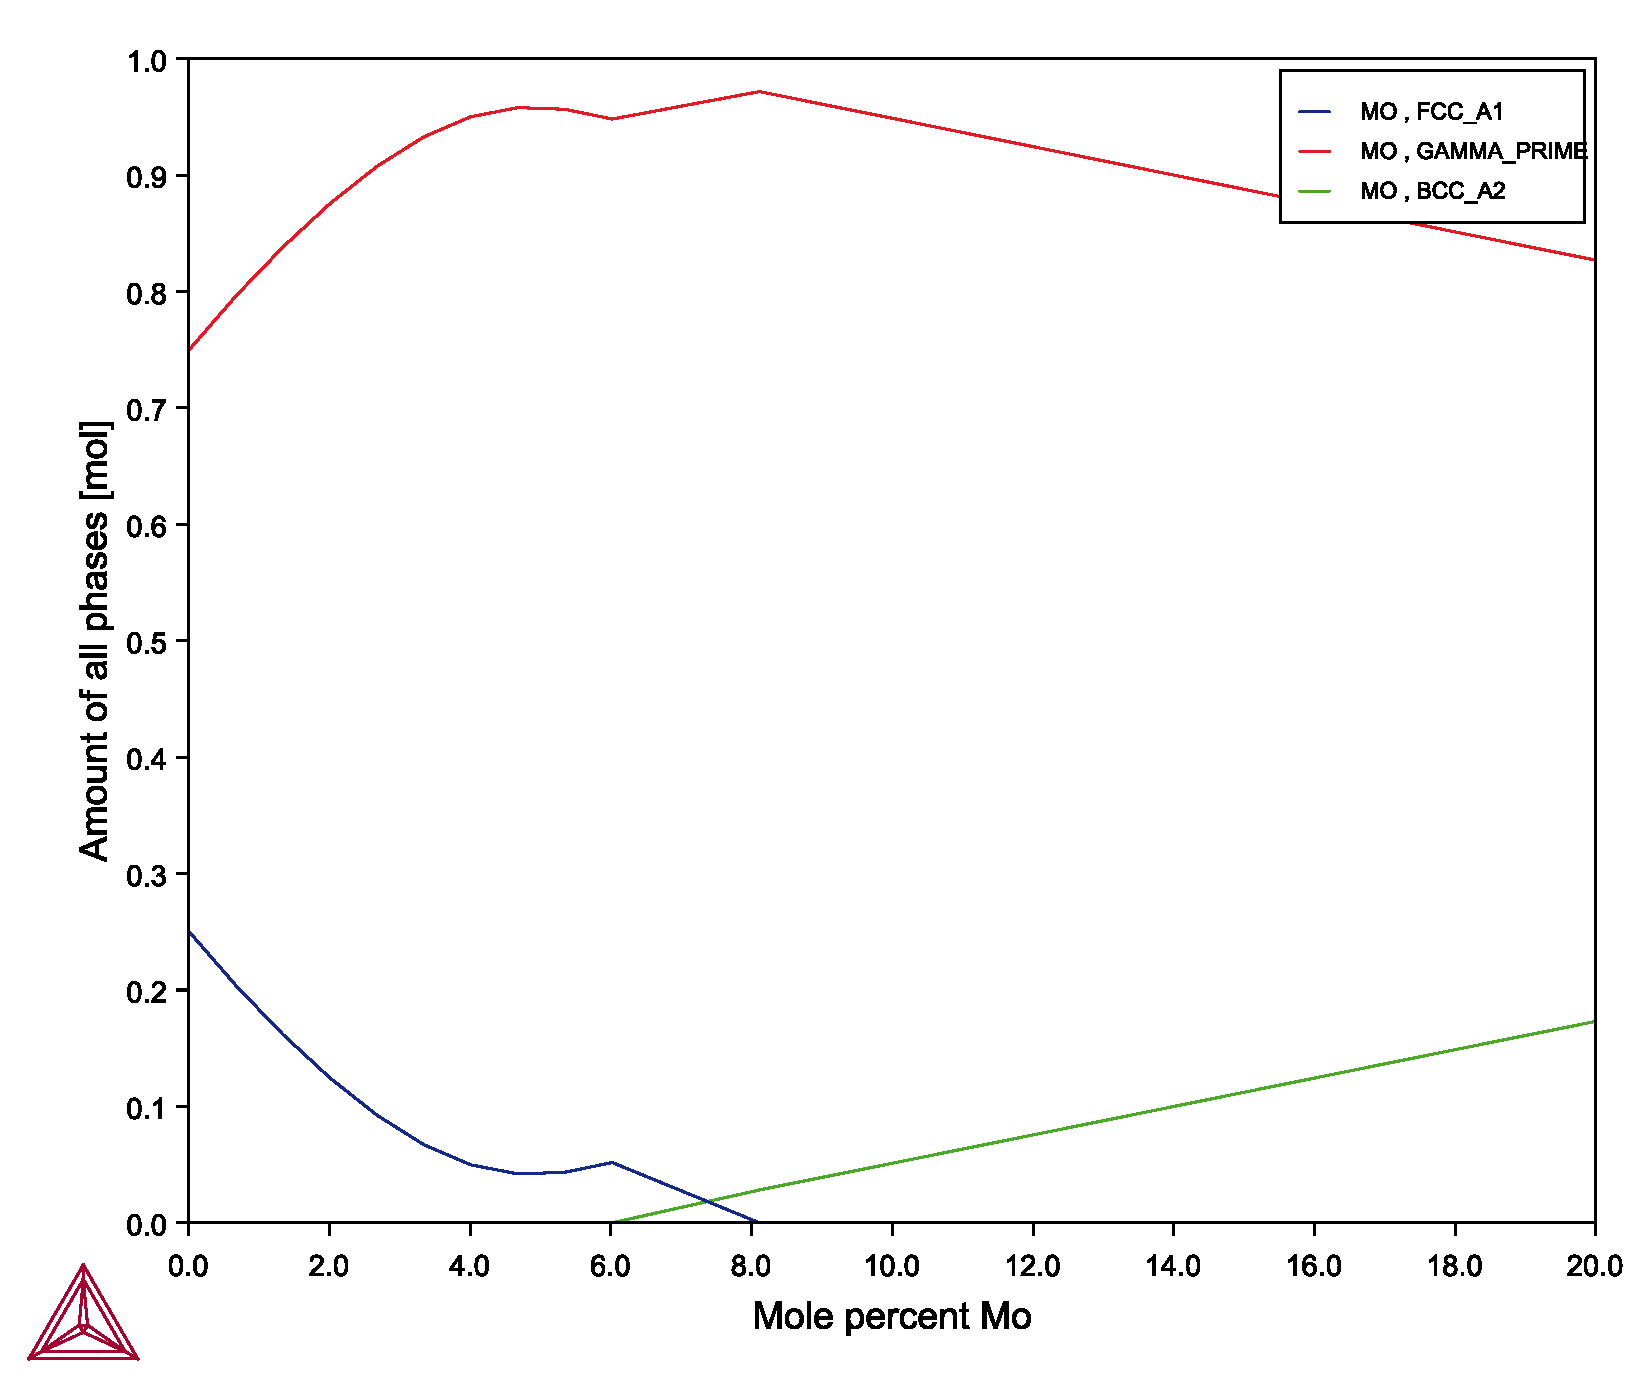
\includegraphics[width=0.5\textwidth]{graficas/Q3_Mo.pdf}} \\
  \subfloat[Re\label{fig:re}]{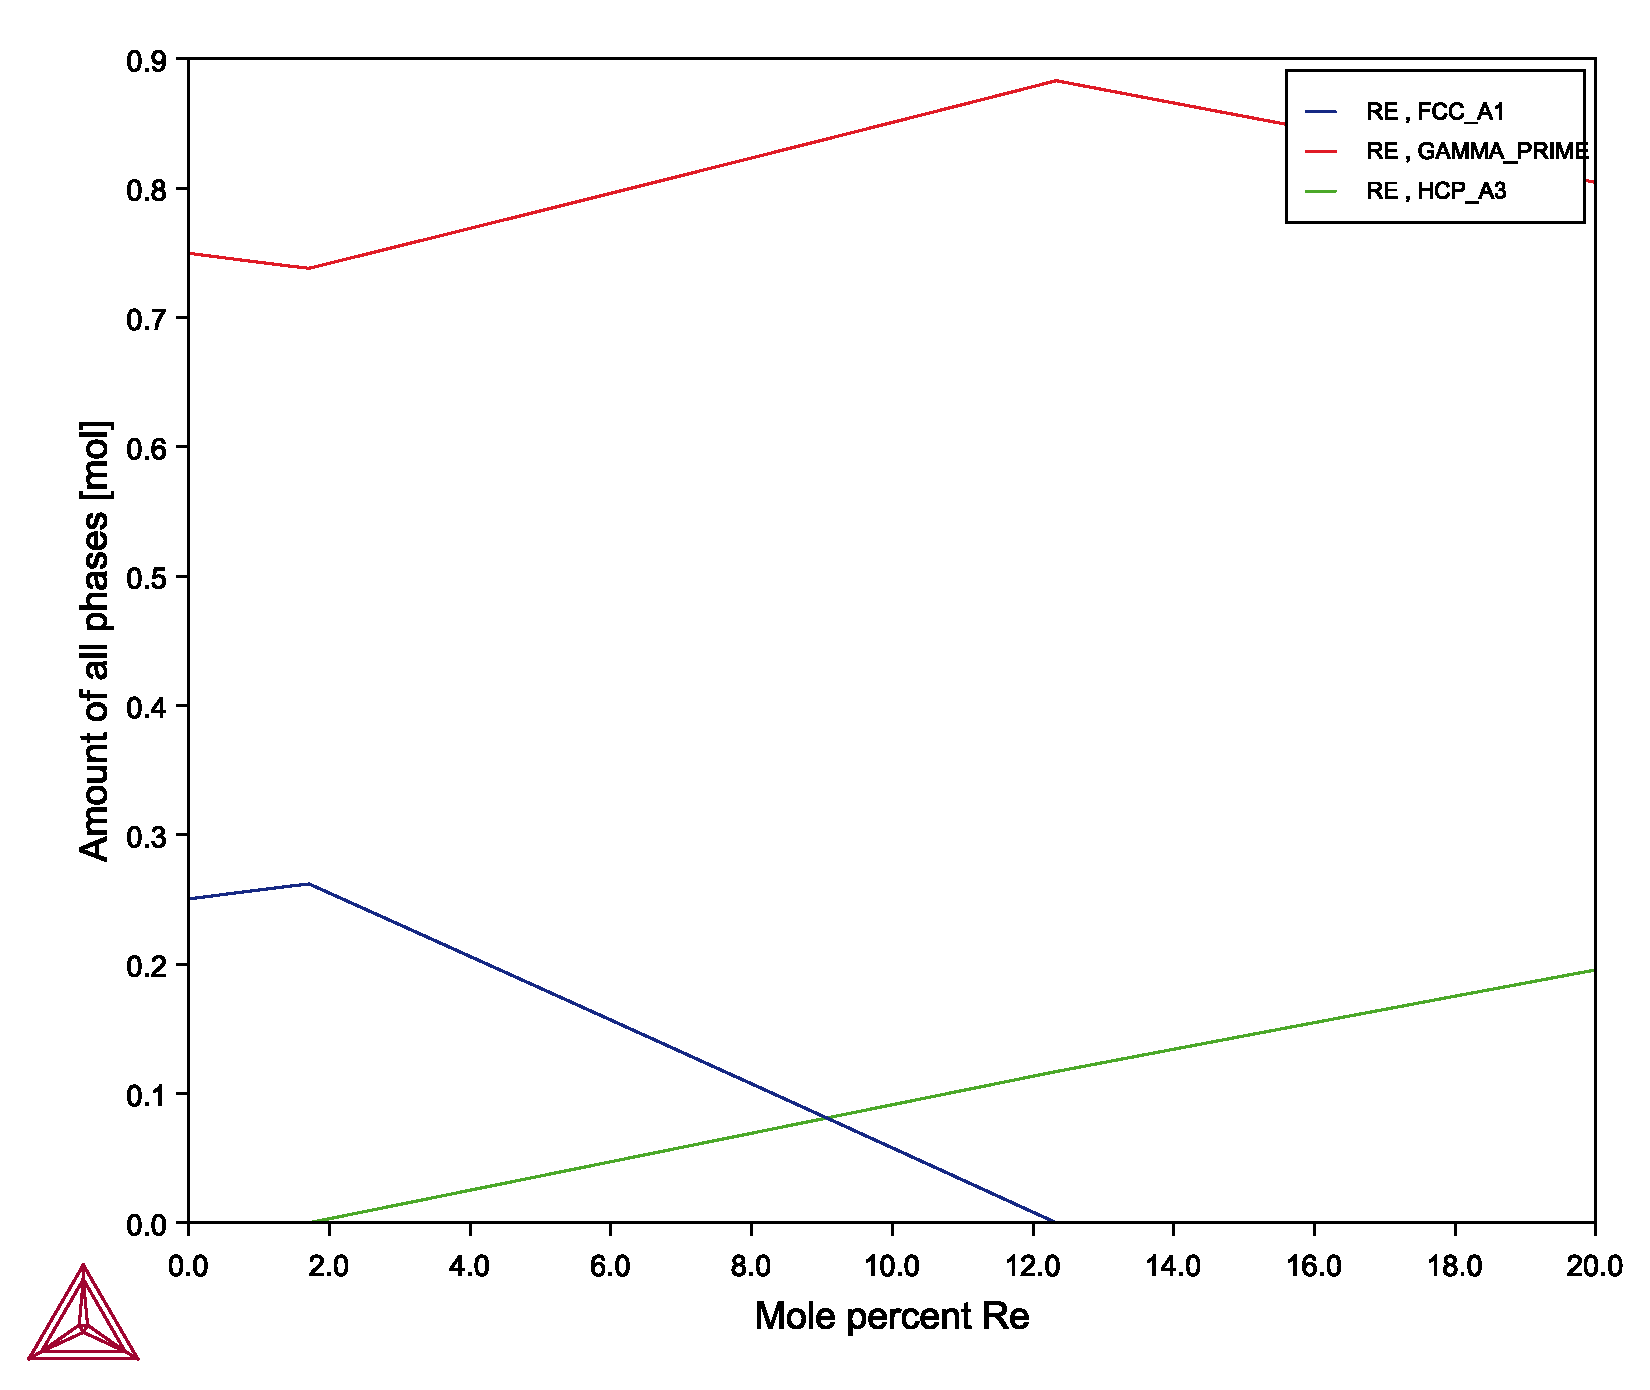
\includegraphics[width=0.5\textwidth]{graficas/Q3_Re.pdf}}
  \subfloat[W\label{fig:w}]{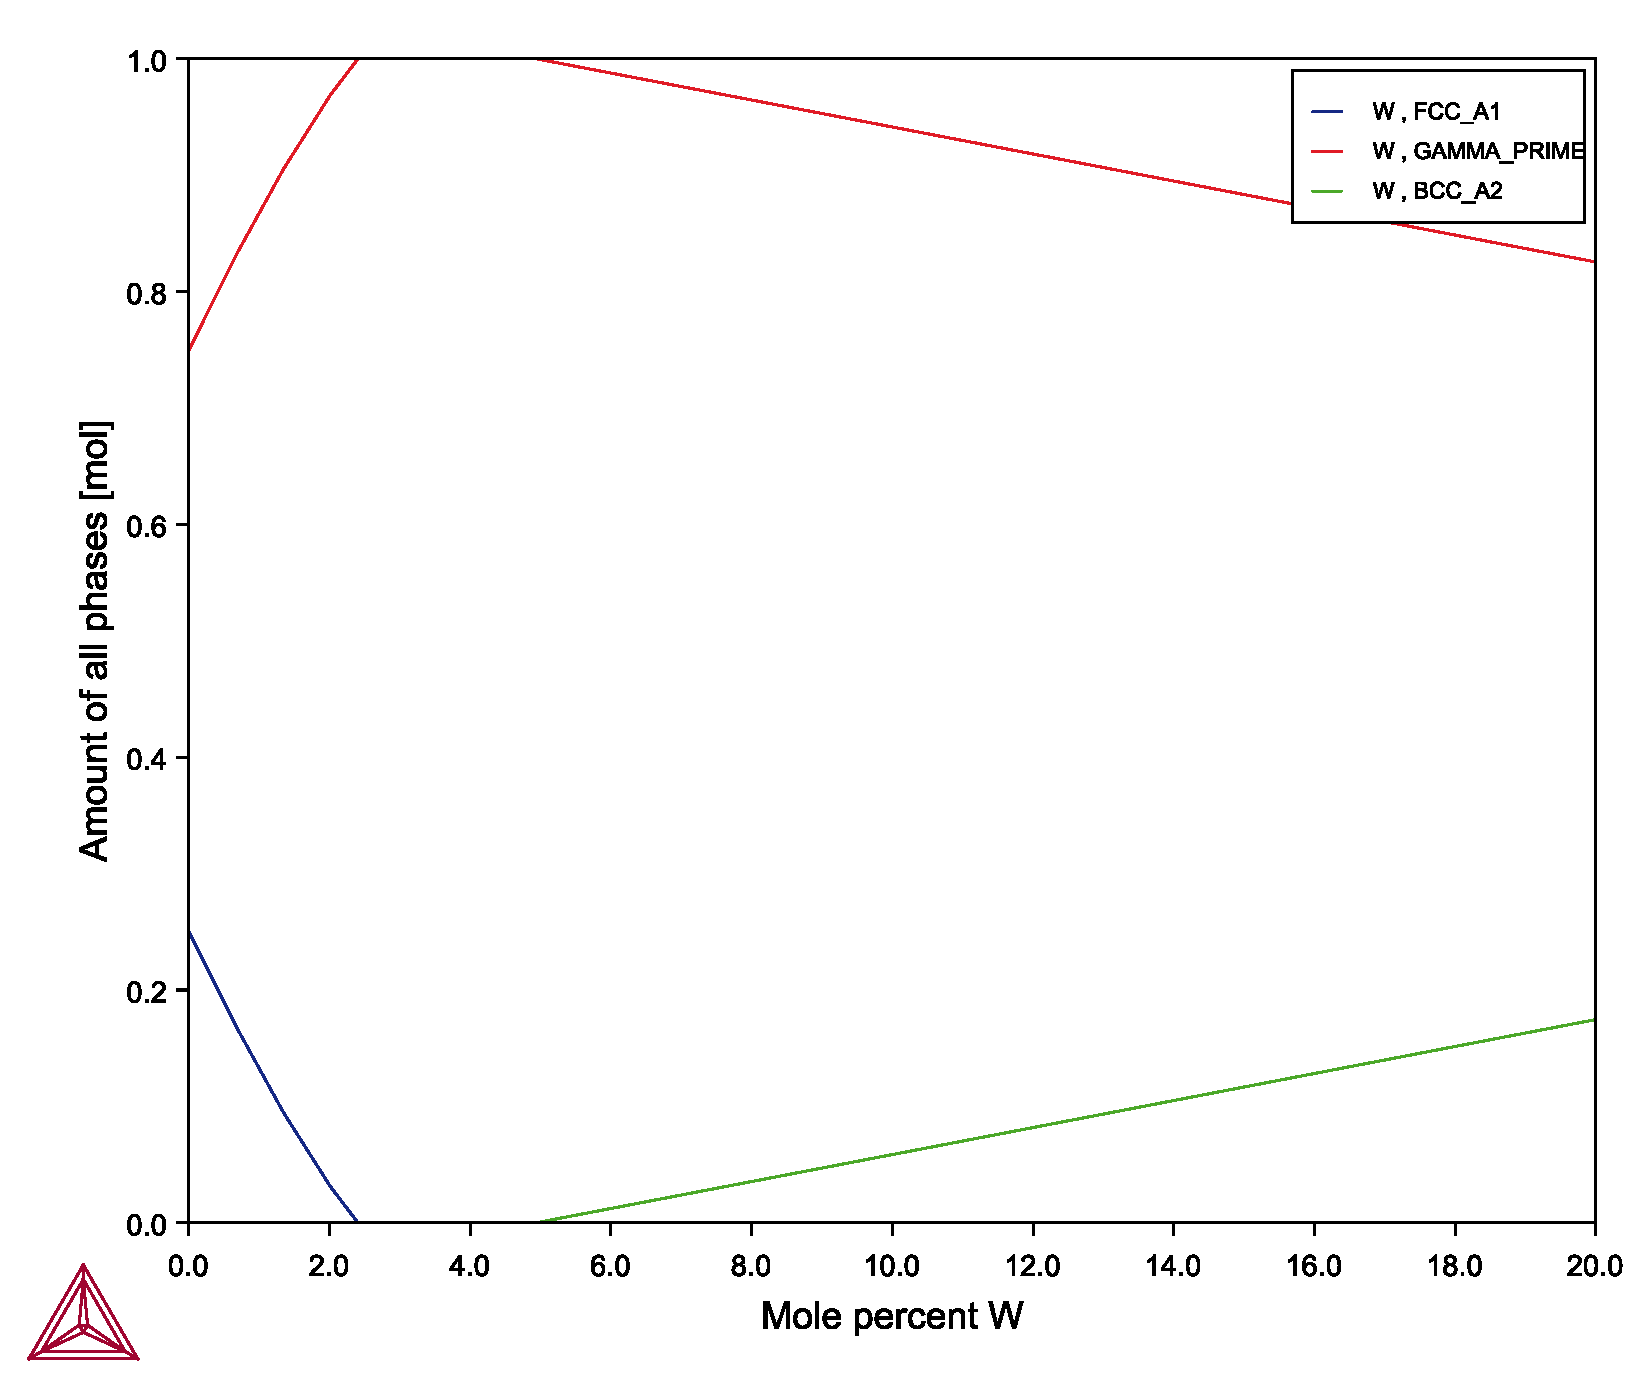
\includegraphics[width=0.5\textwidth]{graficas/Q3_W.pdf}}
  \caption{Amount of phase as function of mole percent of a) Cr, b) Mo, c) Re and d) W generated with \textit{ThermoCalc} \citep{thermocalc}.}
  \label{fig:diagram04}
\end{figure}


\section{}

\subsection{a) Suitable solutioning temperature and extent of the heat treatment window, and b) primary ageing temperature for new alloy}

\textbf{a)} In figure \ref{fig:diagram05} the amount of all phases is plotted as a function of temperature for the alloy system Ni-Al-Ta-Cr-Re-W-Mo. It shows that the $\gamma'$ curve starts at a composition near $0.8$ value and decreases as the temperature increases, reaching a composition of value $0$ around $1388$°C. The temperature where the composition of the $gamma'$ phase becomes zero is the solutioning temperature. 

The liquid curve corresponds to an approximate temperature of $1380$°C, this temperature corresponds to the solidus temperature, where the liquid phase begins to form. 

The hear treatment window corresponds to de window that exists between the solutioning temperature, $1388$°C, to the solidus temperatures, $1380$°C, which gives a window of approximately $8$°C; so in this range of temperature the $\gamma'$ can be dissolved without partial melting of the alloy.

\begin{figure}[h]
  \centering
    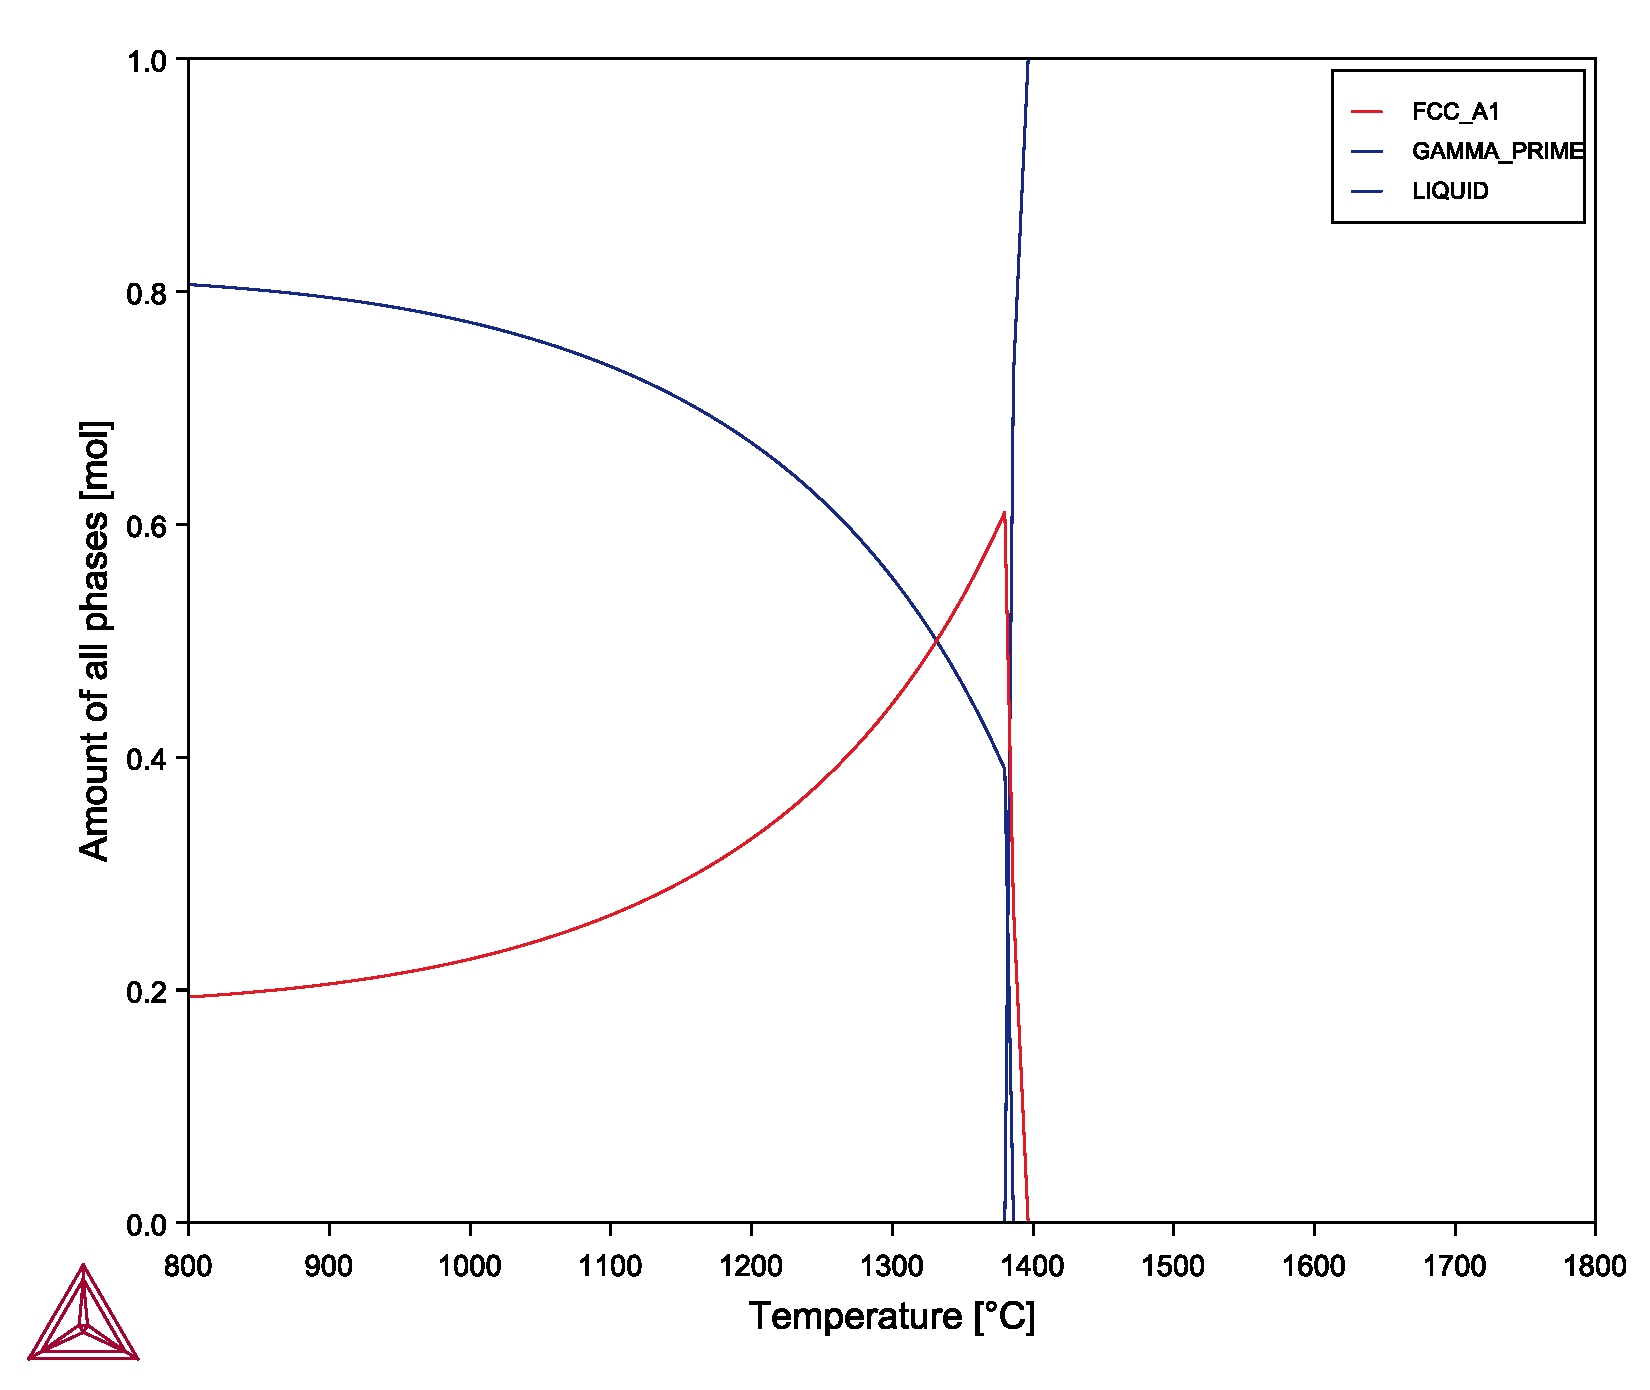
\includegraphics[width=0.95\textwidth]{graficas/Q4_02.pdf}
    \caption{Amount of all phases as a function of temperature generated with \textit{ThermoCalc} \citep{thermocalc}}
    \label{fig:diagram05}
\end{figure}

\textbf{b)} The primary ageing temperature is found at a $\gamma'$ fraction of approximately 0.60, looking at \ref{fig:diagram05} the \shnote{me falta editar la imagen para poder poner ahi el punto donde la curva esta a 0.60}

%The γ′ fraction at lower temperatures is used to define the ageing condition. From the diagram, the γ′ fraction reaches ≈0.60 at a temperature of about 1080 °C. This temperature is therefore selected as the primary ageing temperature, where a stable amount of precipitates can form and strengthen the alloy.

%Why 60% γ′ fraction is used for ageing

%In Ni-based superalloys, the strengthening phase is γ′ (Ni₃Al-type precipitate).

%For good creep resistance and mechanical strength, you want a significant amount of γ′ precipitates but not 100%, because you also need some γ (FCC matrix) for ductility and toughness.

%Experimental alloy design studies have shown that a γ′ volume fraction around 60–70% gives the best balance between strength and workability.
\input{Appendix}
%\section{}

\subsection{a) Suitable solutioning temperature and extent of the heat treatment window, and b) primary ageing temperature for new alloy}

\textbf{a)} In figure \ref{fig:diagram05} the amount of all phases is plotted as a function of temperature for the alloy system Ni-Al-Ta-Cr-Re-W-Mo. It shows that the $\gamma'$ curve starts at a composition near $0.8$ value and decreases as the temperature increases, reaching a composition of value $0$ around $1388$°C. The temperature where the composition of the $gamma'$ phase becomes zero is the solutioning temperature. 

The liquid curve corresponds to an approximate temperature of $1380$°C, this temperature corresponds to the solidus temperature, where the liquid phase begins to form. 

The hear treatment window corresponds to de window that exists between the solutioning temperature, $1388$°C, to the solidus temperatures, $1380$°C, which gives a window of approximately $8$°C; so in this range of temperature the $\gamma'$ can be dissolved without partial melting of the alloy.

\begin{figure}[h]
  \centering
    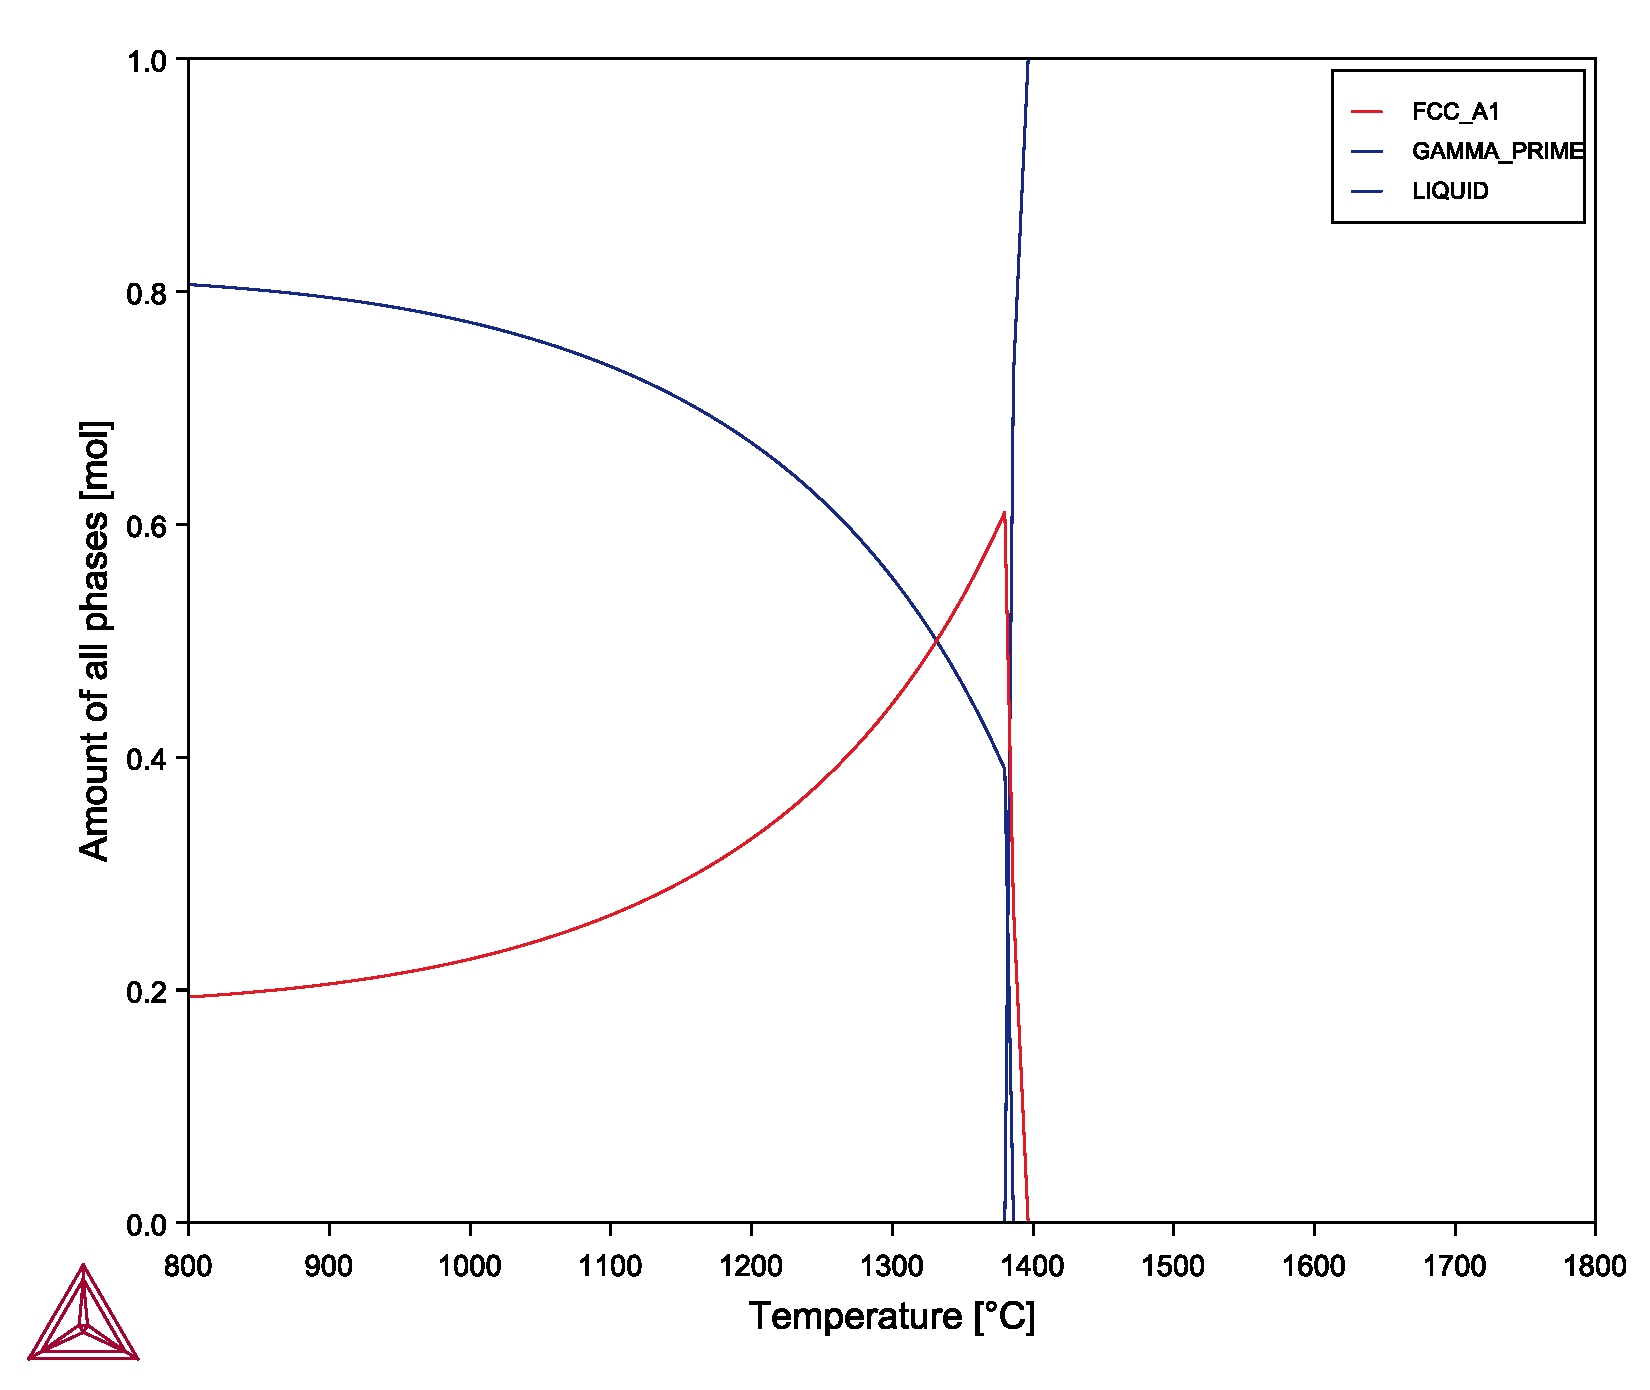
\includegraphics[width=0.95\textwidth]{graficas/Q4_02.pdf}
    \caption{Amount of all phases as a function of temperature generated with \textit{ThermoCalc} \citep{thermocalc}}
    \label{fig:diagram05}
\end{figure}

\textbf{b)} The primary ageing temperature is found at a $\gamma'$ fraction of approximately 0.60, looking at \ref{fig:diagram05} the \shnote{me falta editar la imagen para poder poner ahi el punto donde la curva esta a 0.60}

%The γ′ fraction at lower temperatures is used to define the ageing condition. From the diagram, the γ′ fraction reaches ≈0.60 at a temperature of about 1080 °C. This temperature is therefore selected as the primary ageing temperature, where a stable amount of precipitates can form and strengthen the alloy.

%Why 60% γ′ fraction is used for ageing

%In Ni-based superalloys, the strengthening phase is γ′ (Ni₃Al-type precipitate).

%For good creep resistance and mechanical strength, you want a significant amount of γ′ precipitates but not 100%, because you also need some γ (FCC matrix) for ductility and toughness.

%Experimental alloy design studies have shown that a γ′ volume fraction around 60–70% gives the best balance between strength and workability.
%\nocite{*}
\clearpage
\bibliography{references}


% --------------------------------------------------------------
%     You don't have to mess with anything below this line.
% -------------------------------------------------------------- 
\end{document}